\documentclass[assd_guia_filtros_recursivos_main.tex]{subfiles}

\begin{document}

\section{Ejercicio 6}
Mostramos a continuación resultados seleccionados de filtros butterworth y chebycheff con
$f_p=f_s/\alpha$, $f_s=10kHz$, $A_p=2db$


\subsection{Método invariante al impulso}

\begin{figure}[H]	
	\centering
	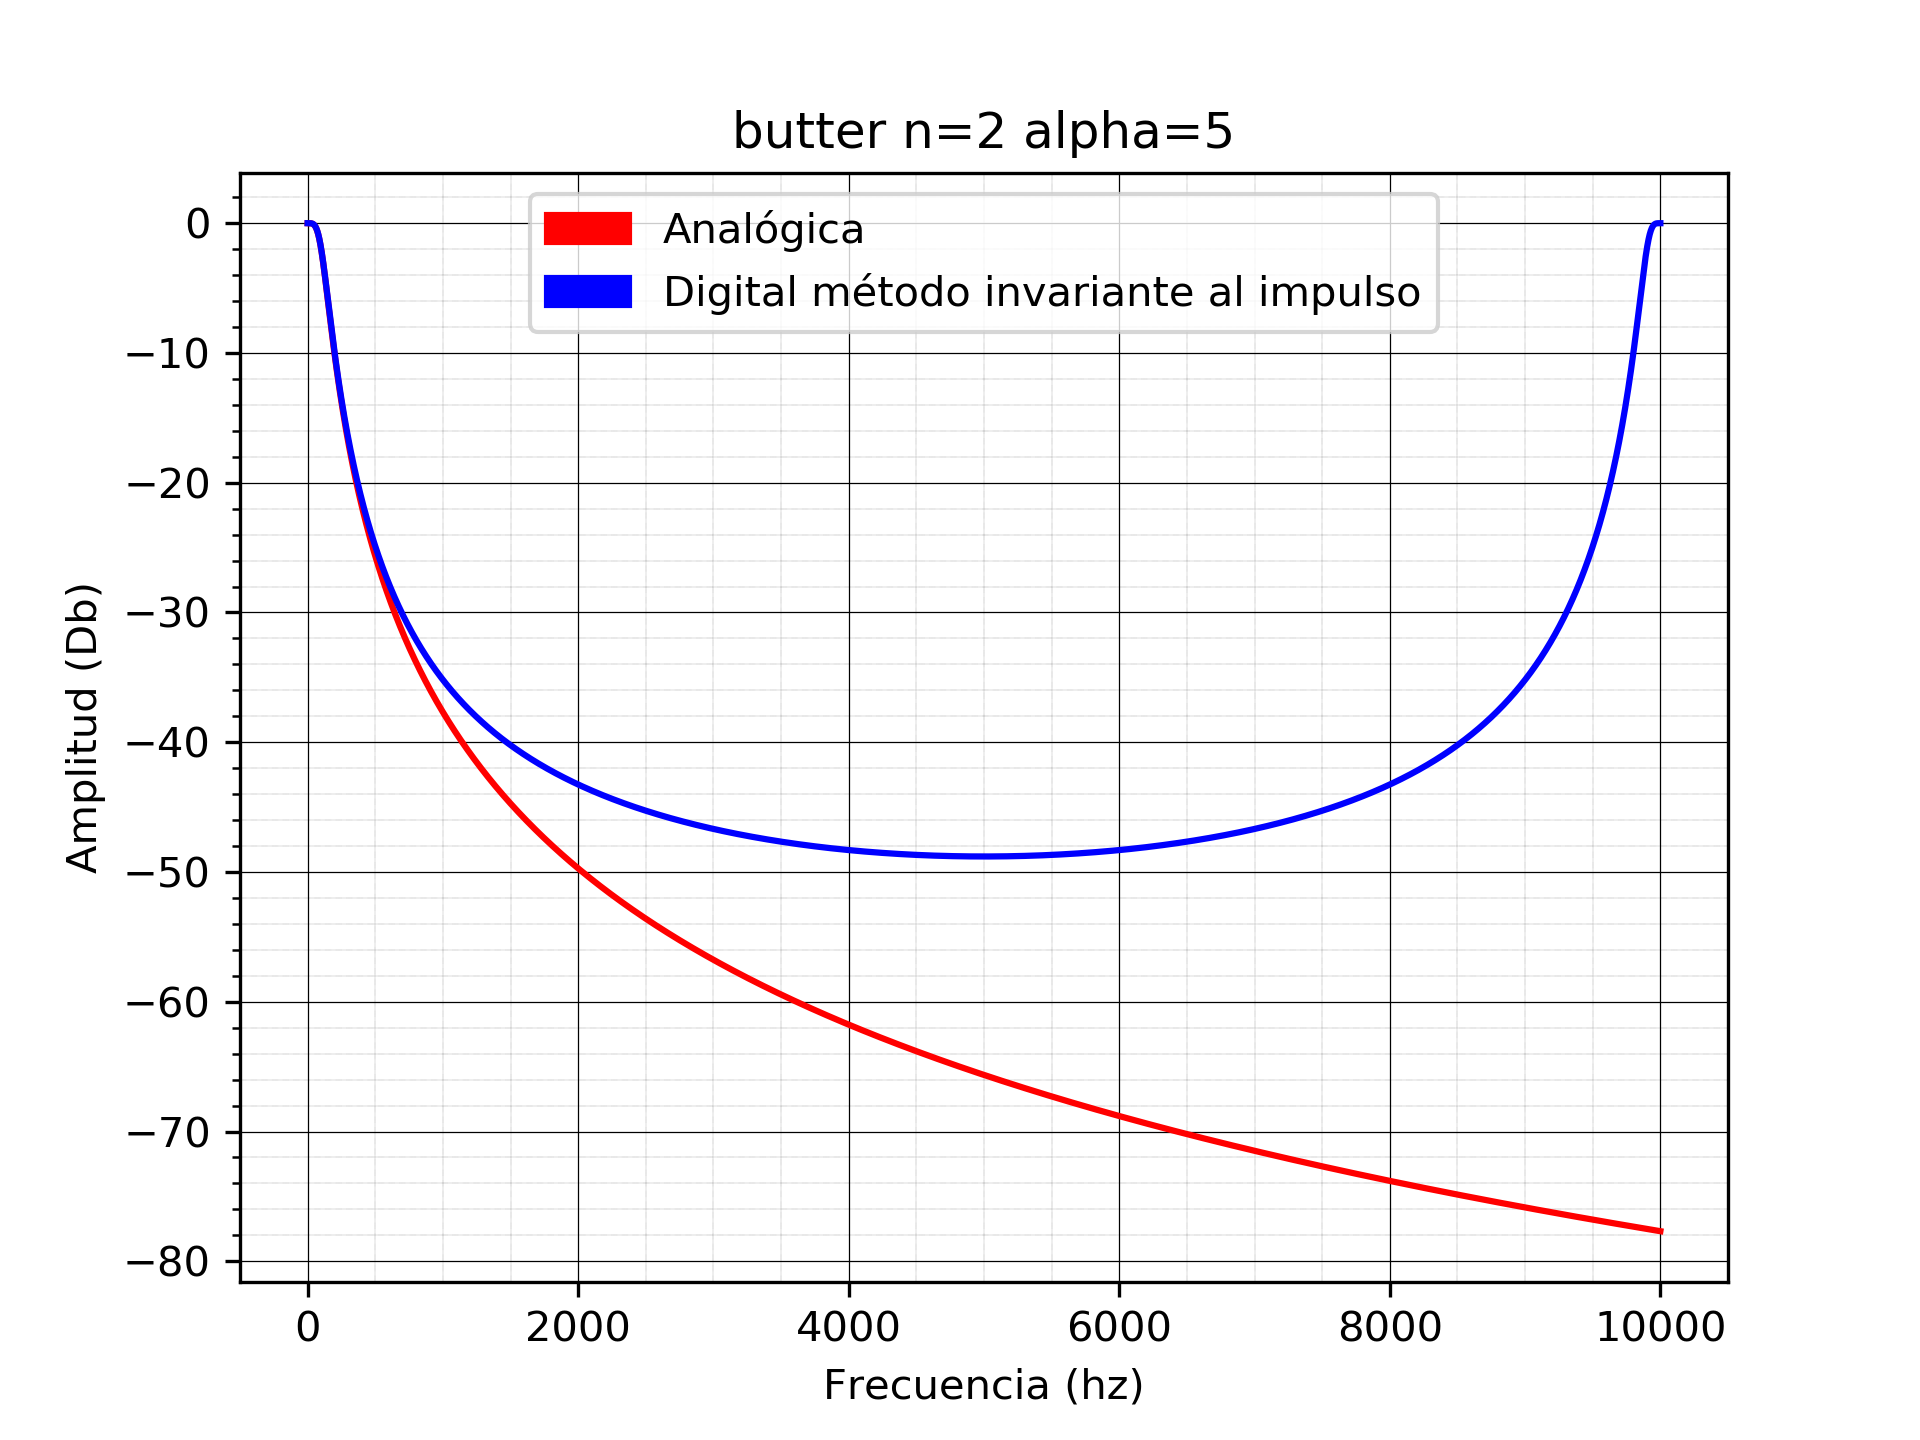
\includegraphics[scale=0.4]{output/butter/alpha=5/butter_n=2.png}
	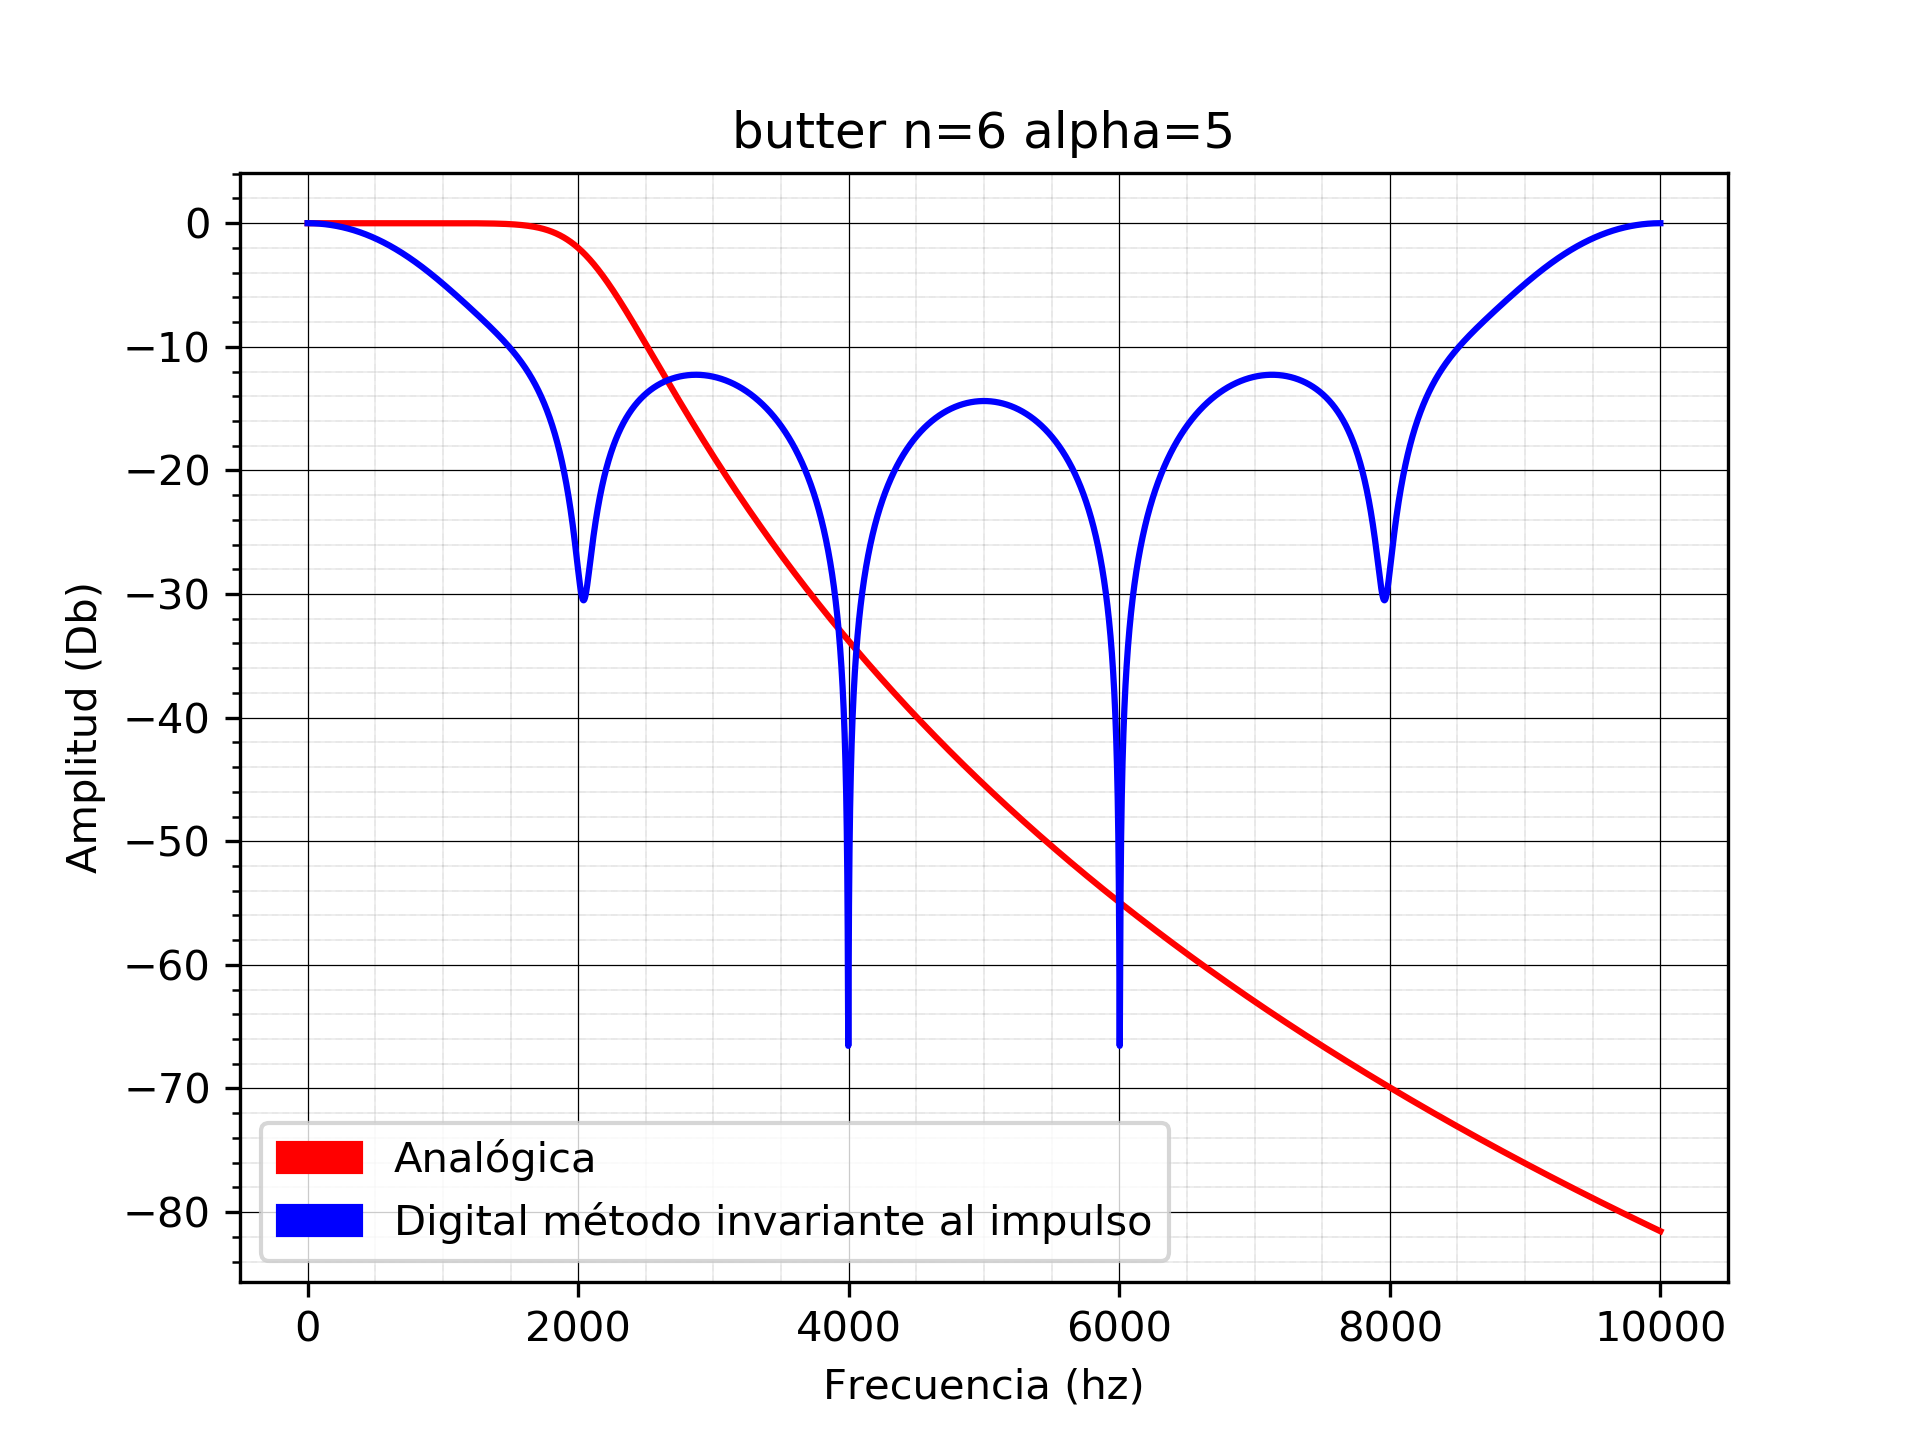
\includegraphics[scale=0.4]{output/butter/alpha=5/butter_n=6.png}
	\caption{Ejemplo Butter n=2, n=6 método invariante al impulso}
	\label{fig:Caso 1}
\end{figure}

Se observa que como $f_p$ estuvo muy cerca de $f_s$ no fue adecuada la transformación.

\begin{figure}[H]	
	\centering
	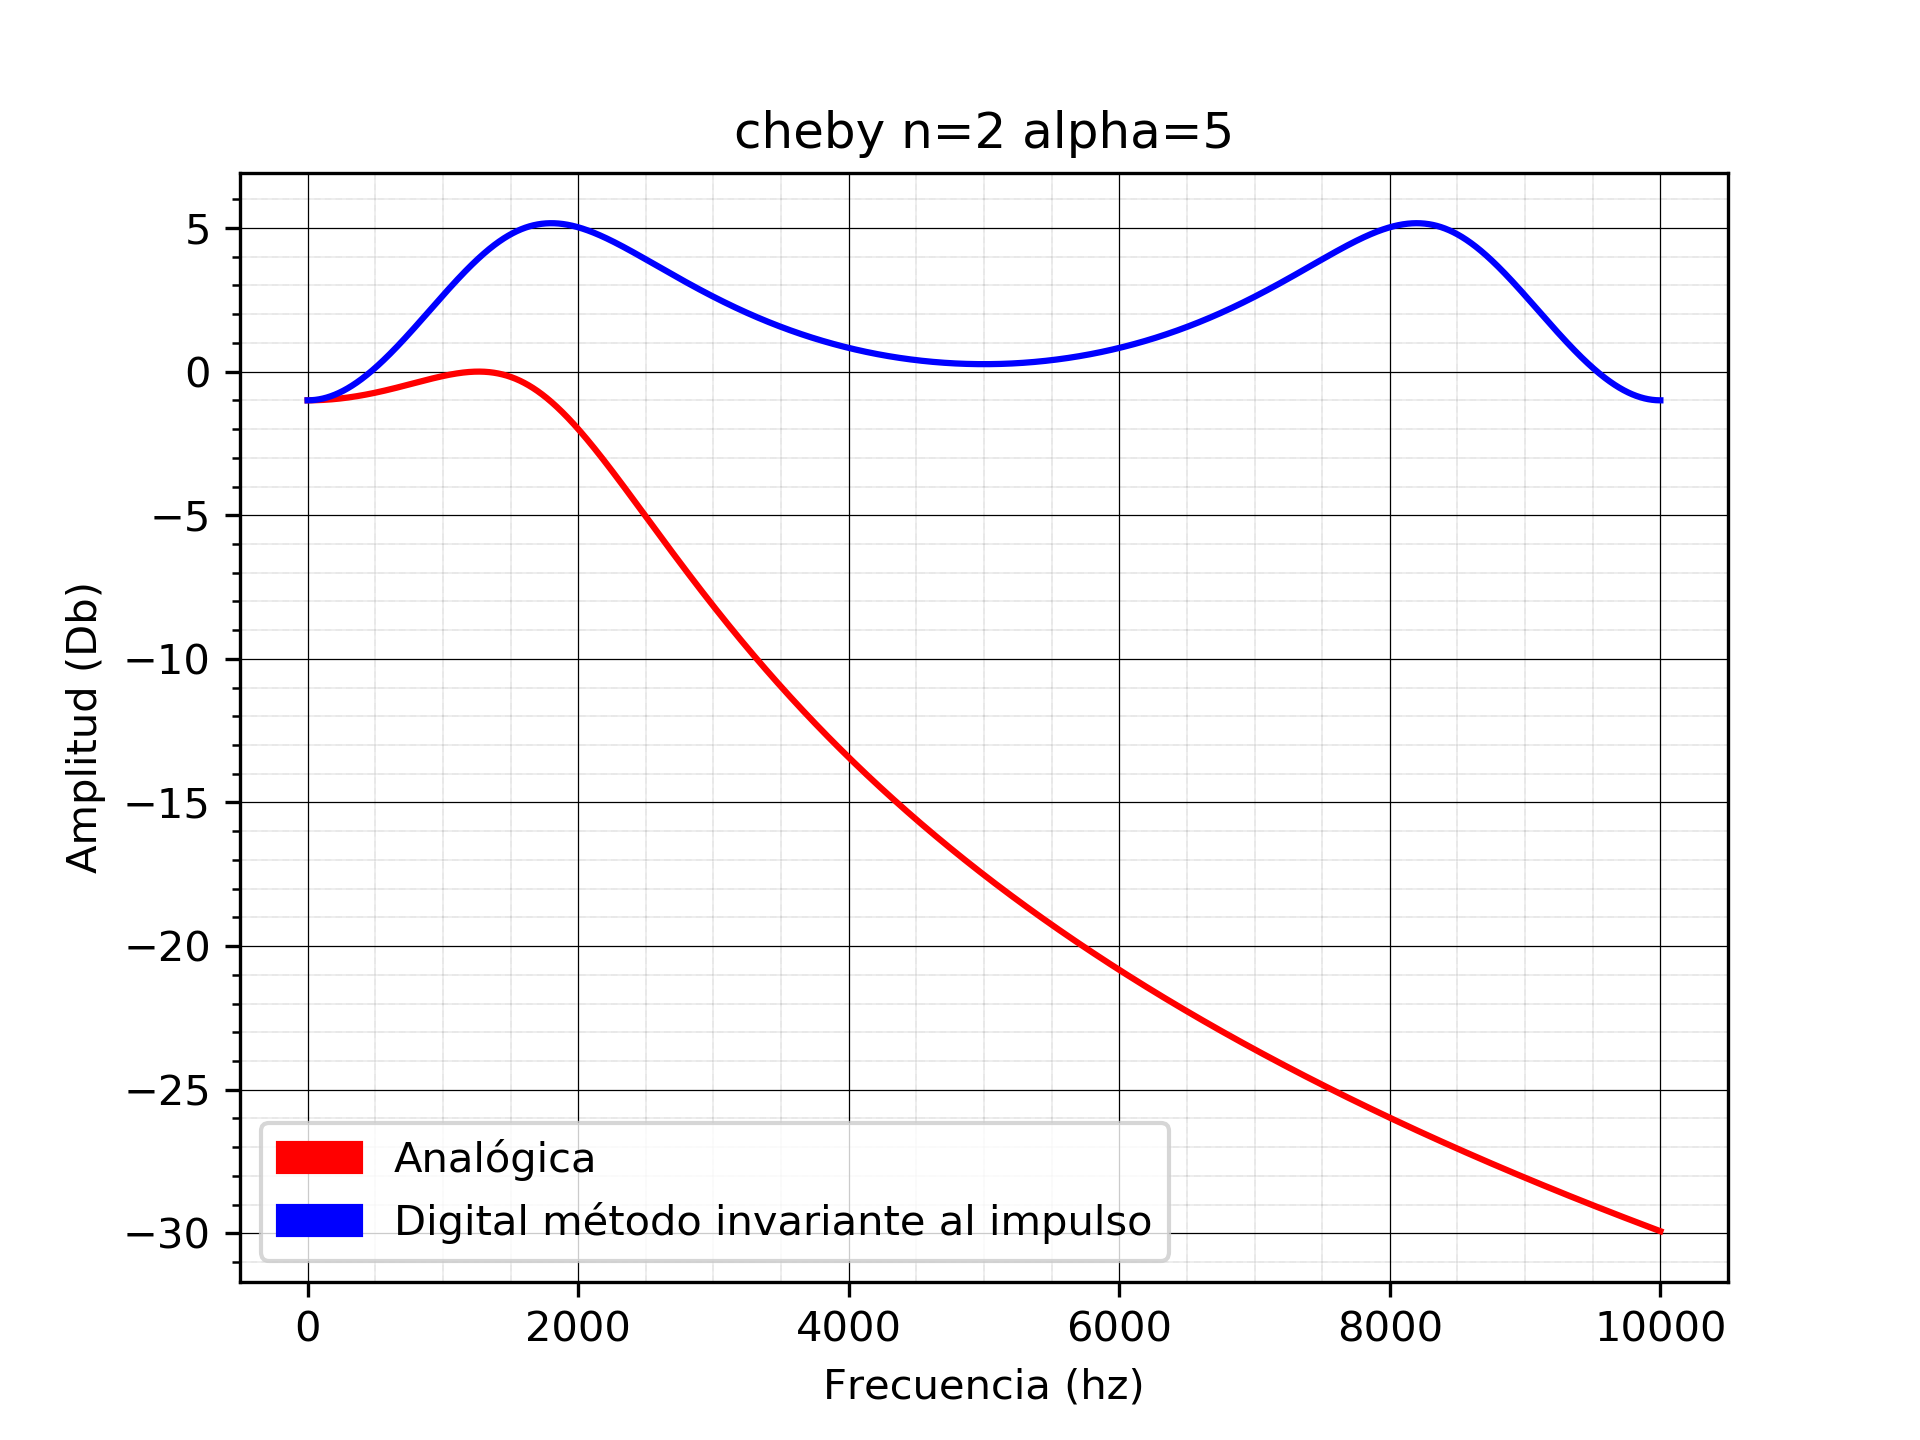
\includegraphics[scale=0.4]{output/cheby/alpha=5/cheby_n=2.png}
	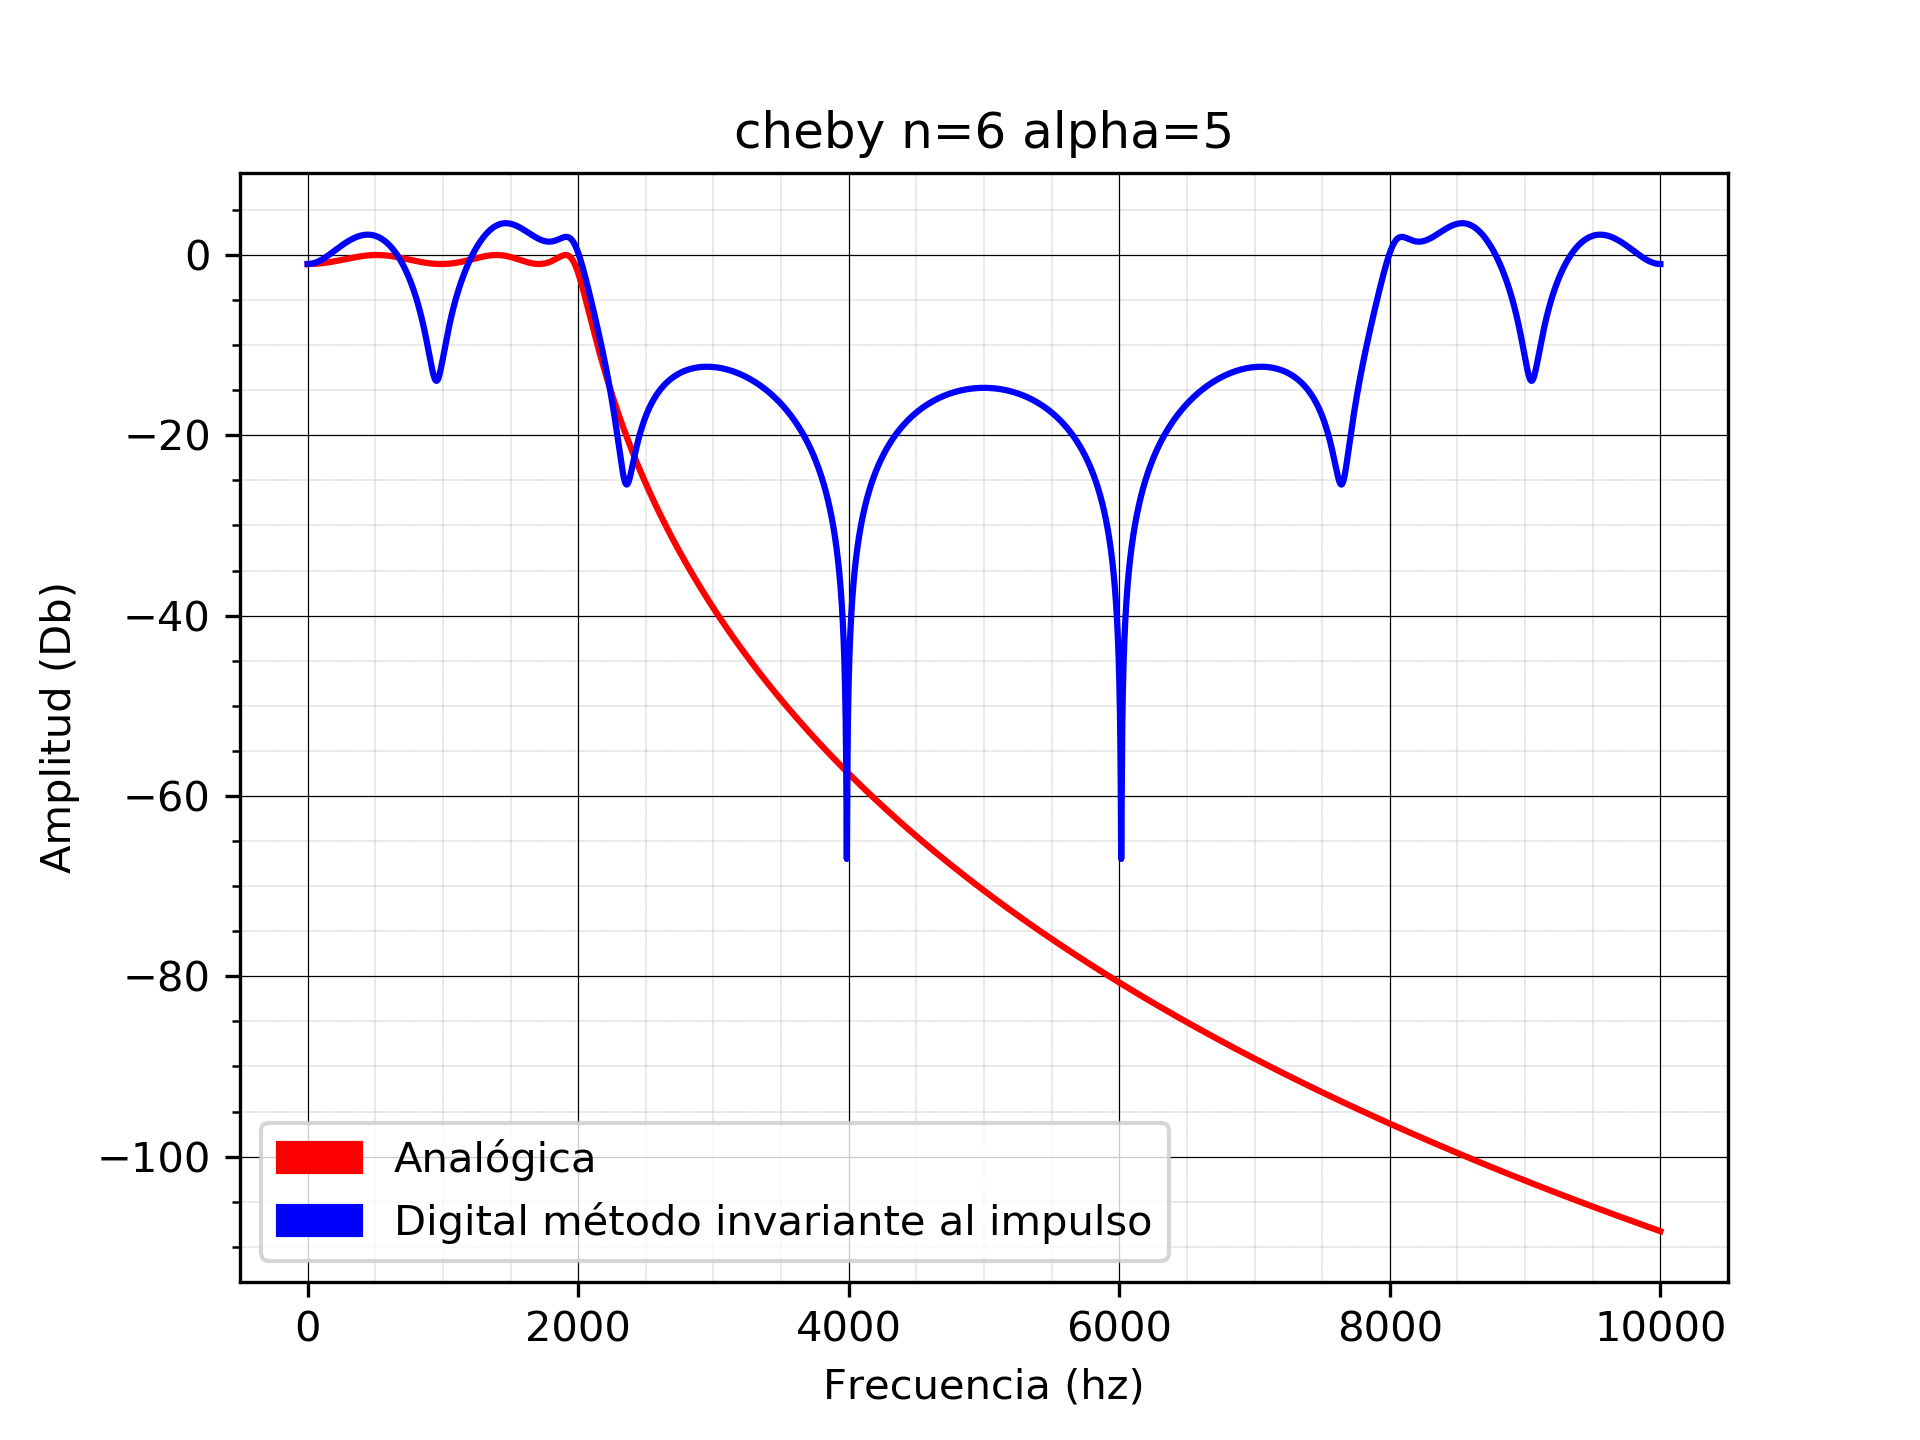
\includegraphics[scale=0.4]{output/cheby/alpha=5/cheby_n=6.png}
	\caption{Ejemplo Cheby n=2, n=6 método invariante al impulso}
	\label{fig:Caso 2}
\end{figure}

Con el filtro chebycheff los resultados fueron equivalentes, no es conveniente que $f_s$ sea comparable con $f_p$

\subsection{Método Matched Z}
A continuación mostramos los resultados aplicando el método matched z

\begin{figure}[H]	
	\centering
	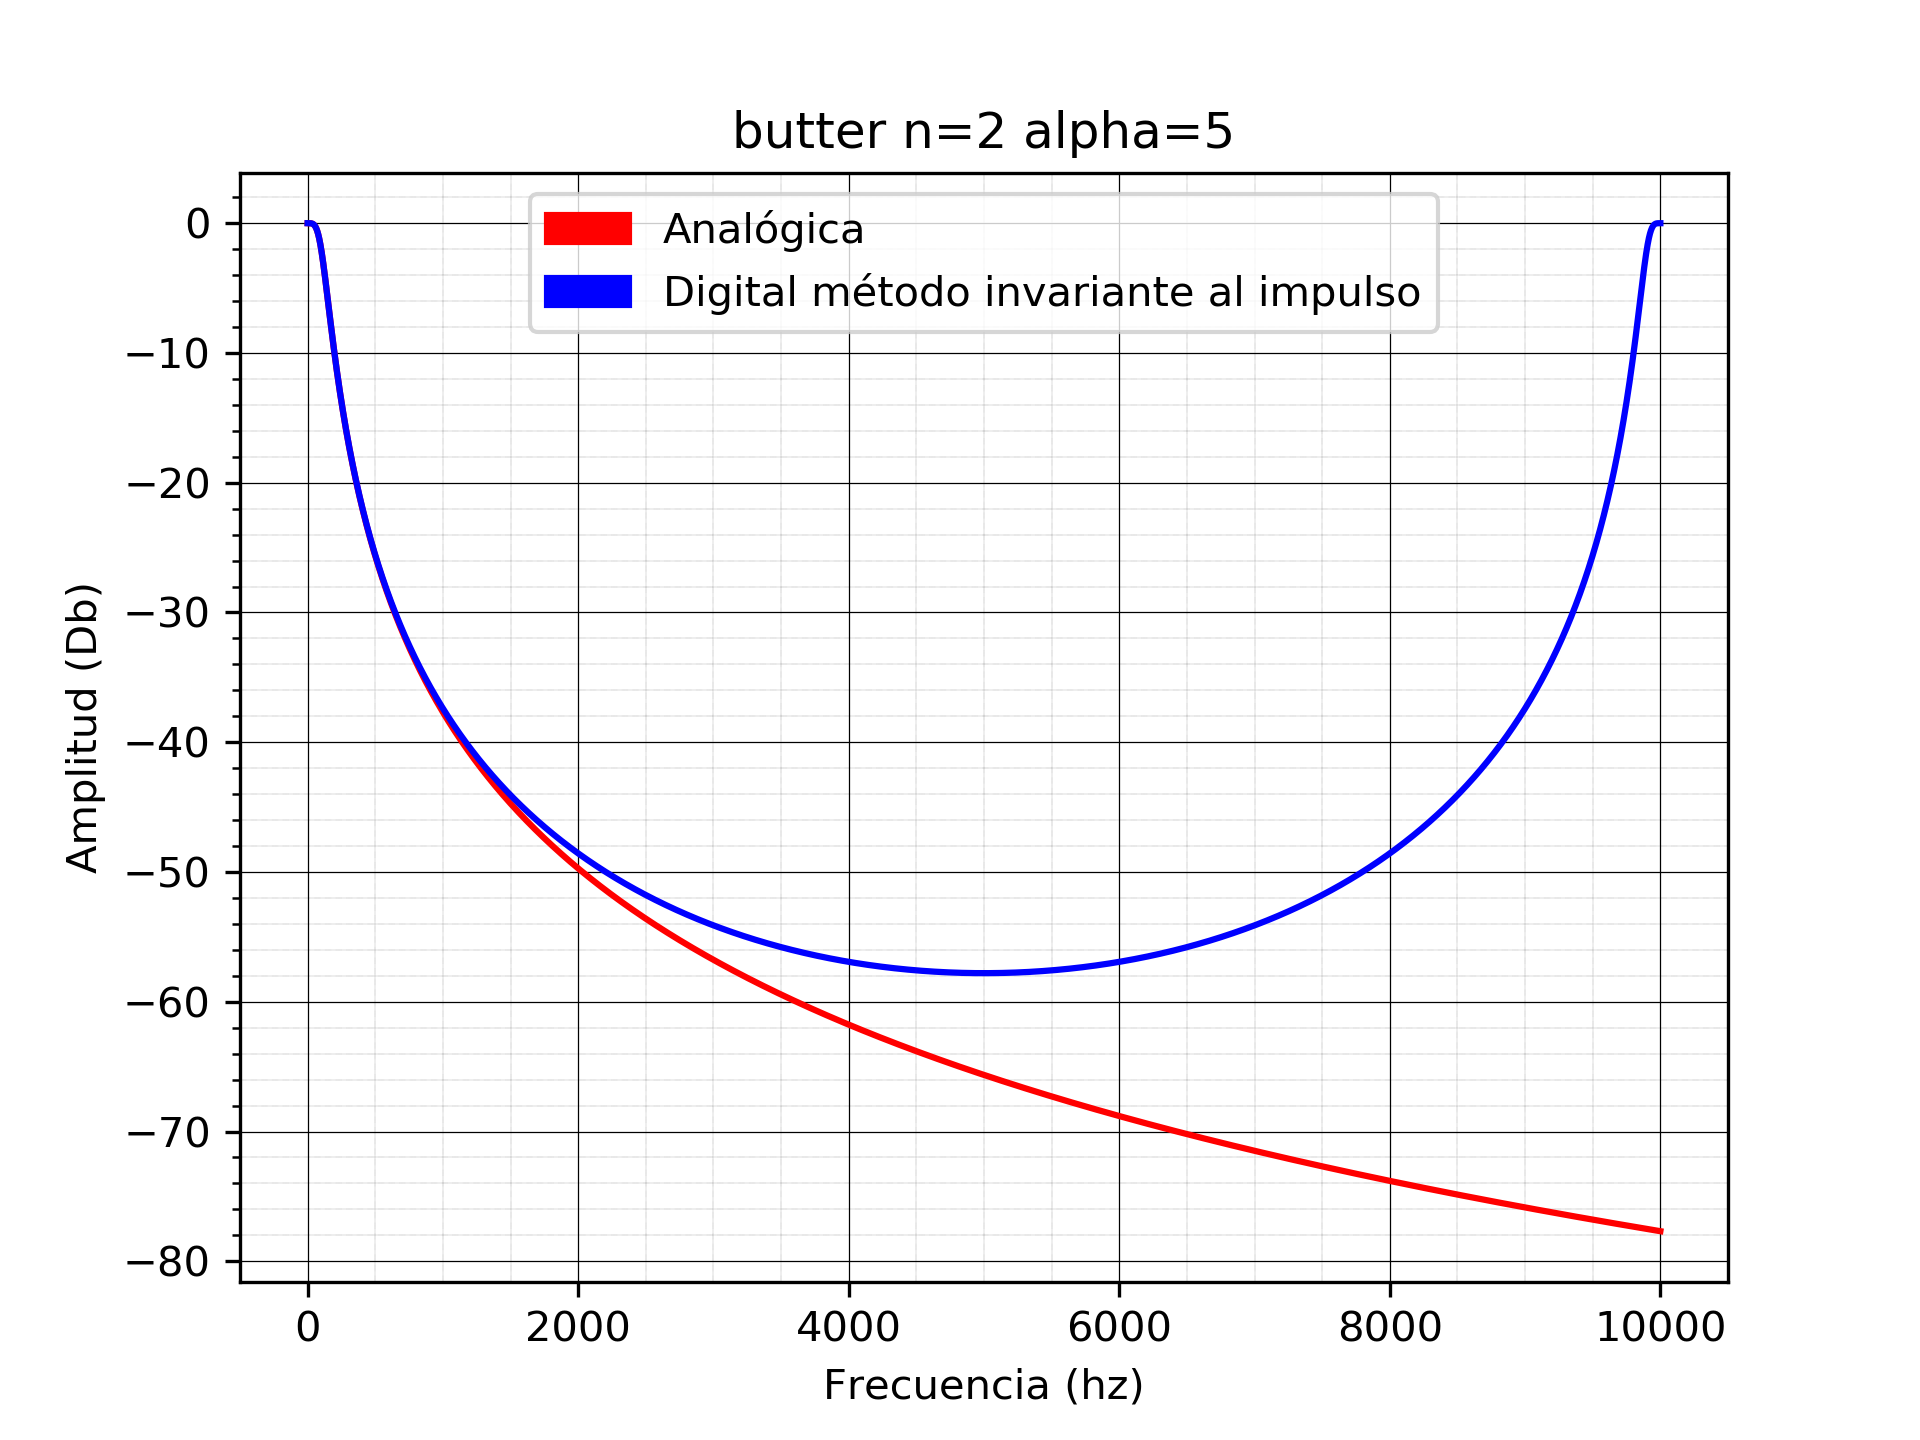
\includegraphics[scale=0.4]{output/butter_matched_z/alpha=5/butter_n=2.png}
	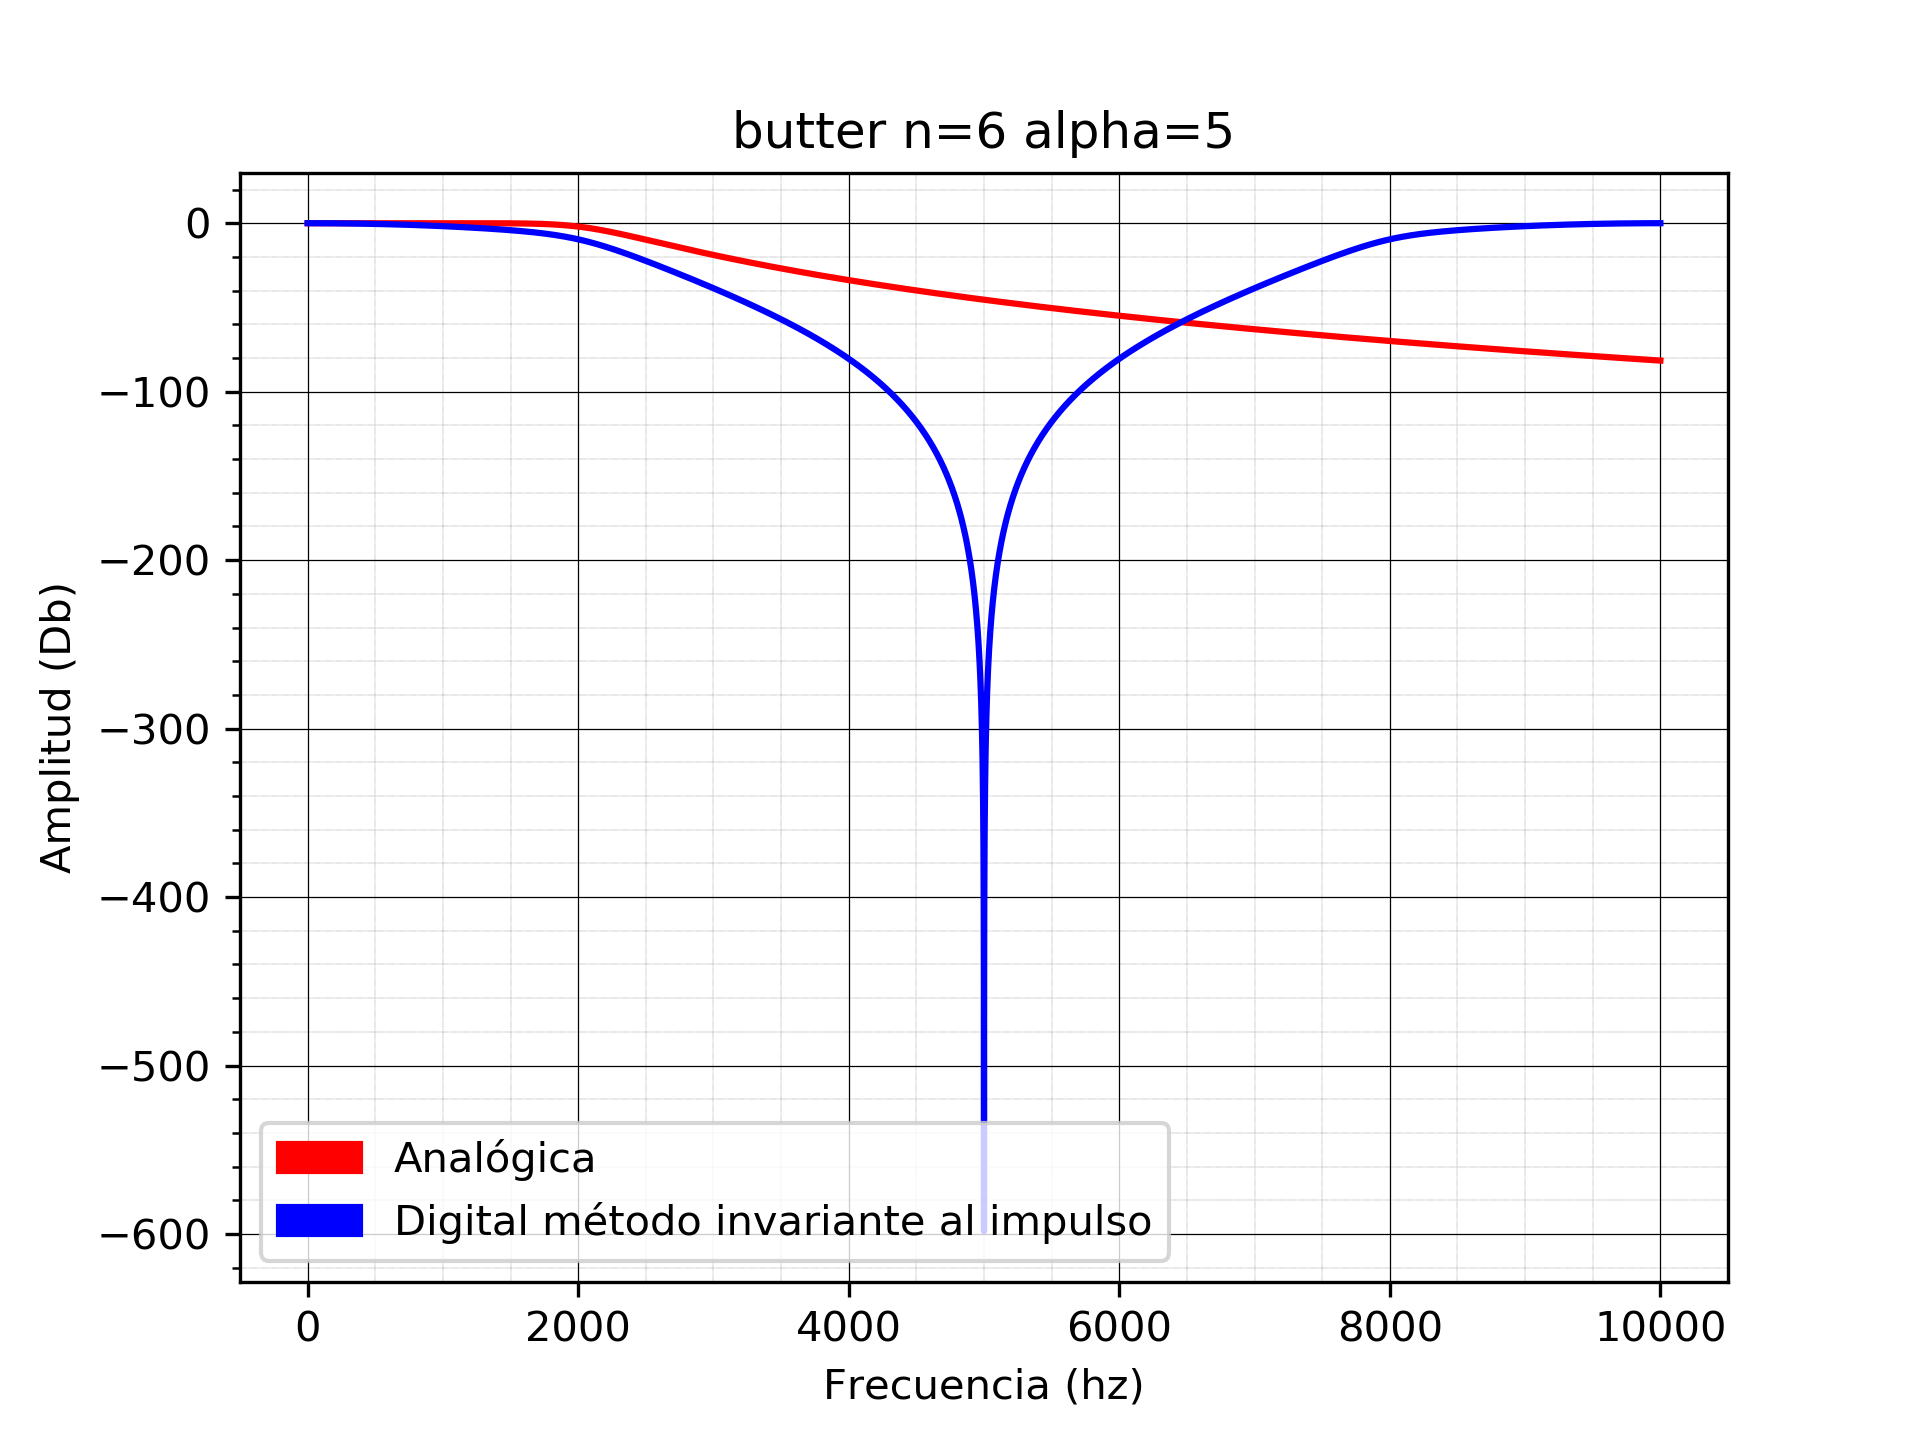
\includegraphics[scale=0.4]{output/butter_matched_z/alpha=5/butter_n=6.png}
	\caption{Ejemplo Butter n=2, n=6 método matched Z}
	\label{fig:Caso 3}
\end{figure}

Con la utilización del método matched Z no se observaron los ceros de transmisión que con el método invariante al impulso si. Los resultados fueron un poco mejor que en el caso anterior ya que en la banda atenuada existió mayor atenuación, no obstante como $f_s$ sigue siendo comparable con $f_p$ no es suficientemente buena la transformación.

\begin{figure}[H]	
	\centering
	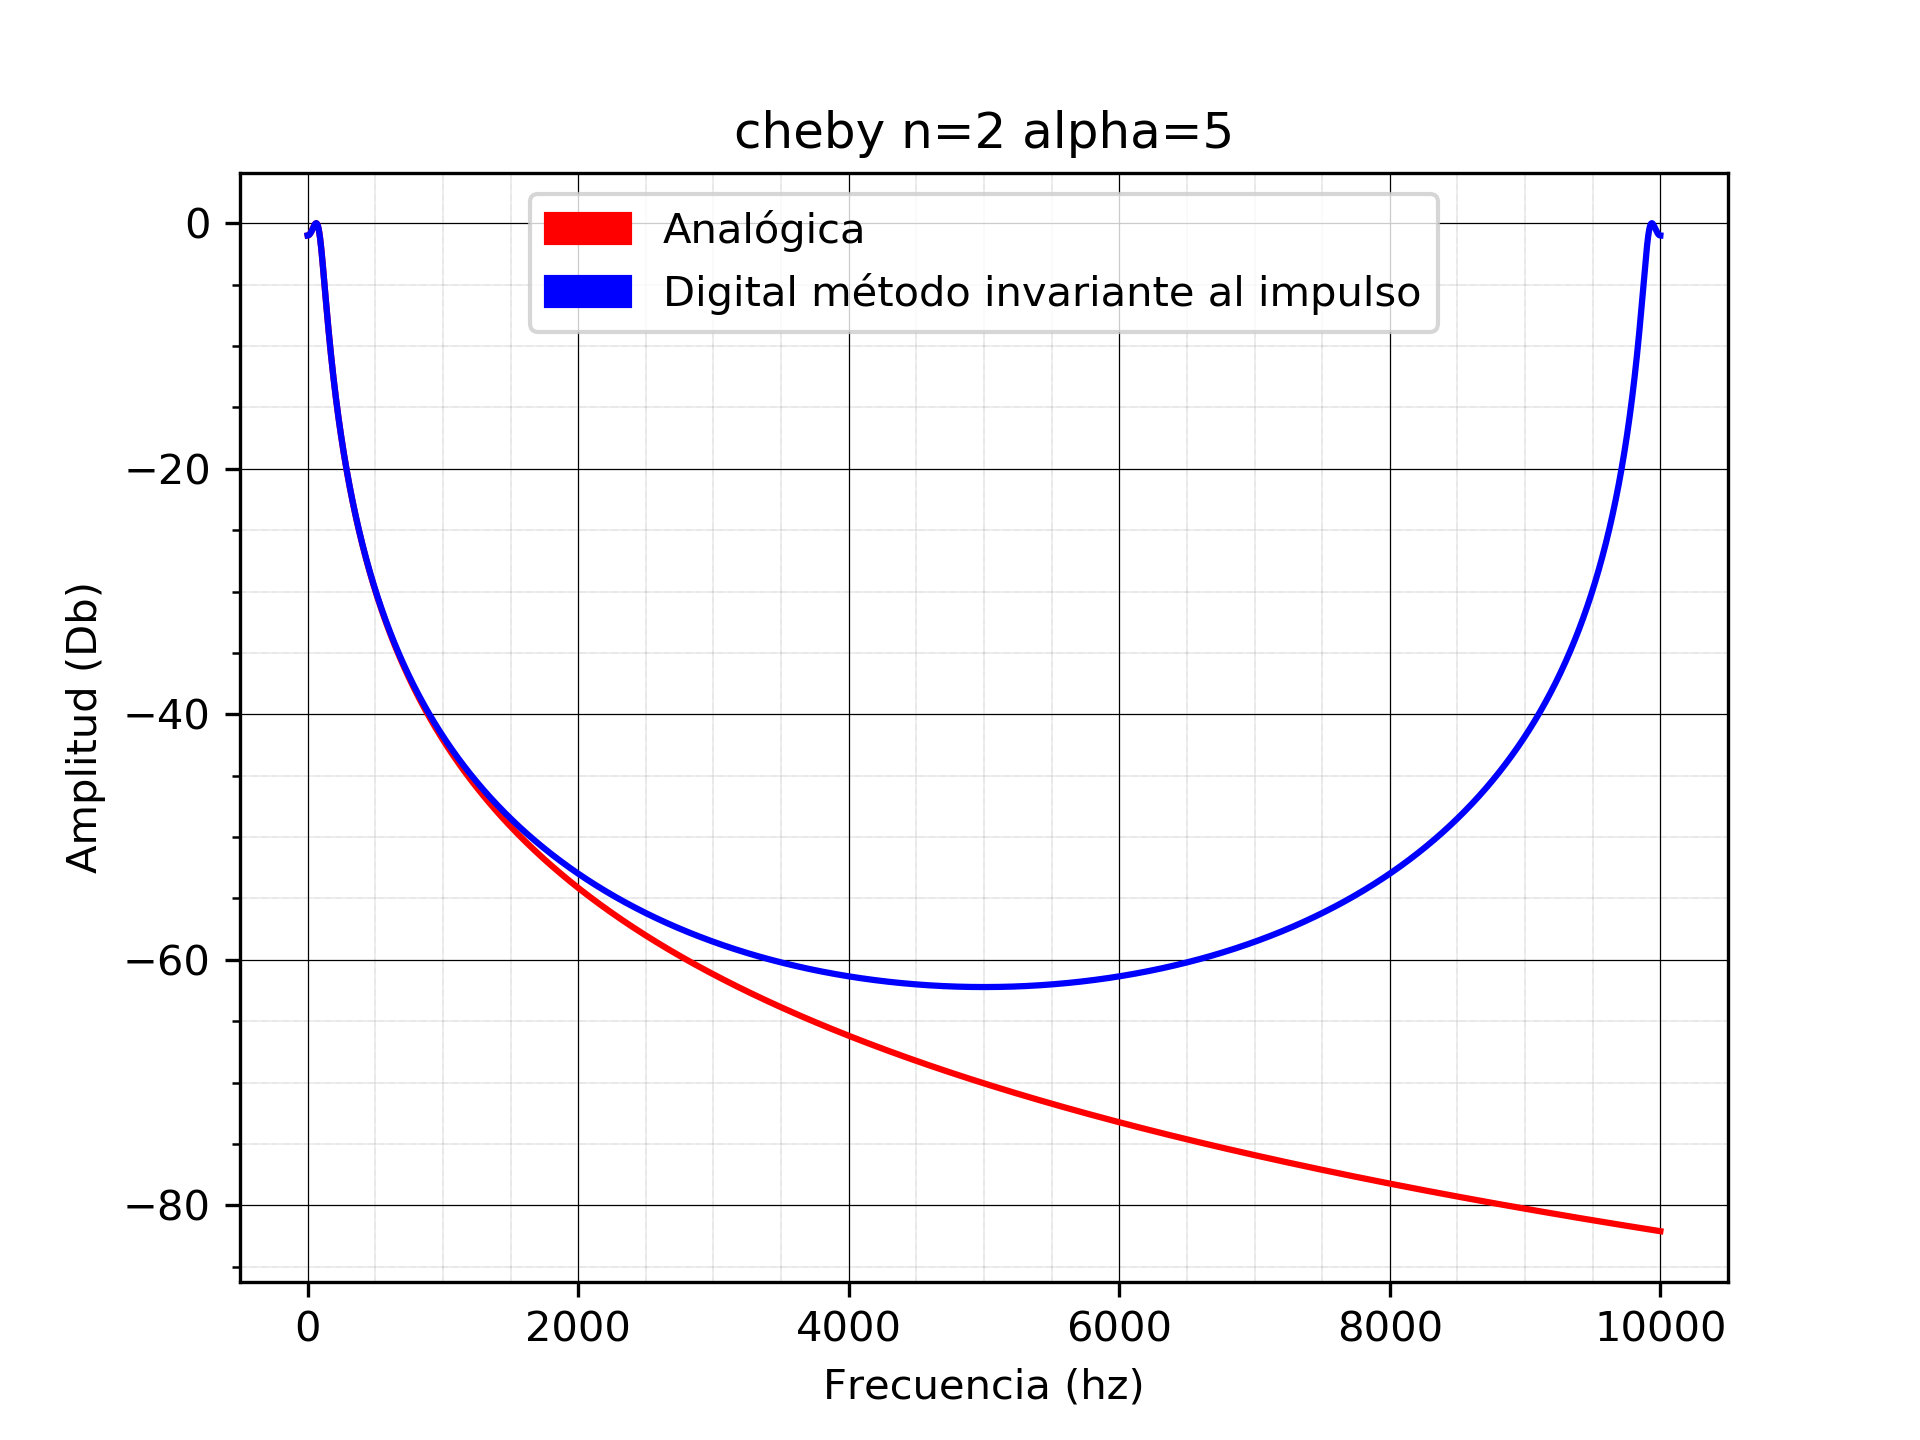
\includegraphics[scale=0.4]{output/cheby_matched_z/alpha=5/cheby_n=2.png}
	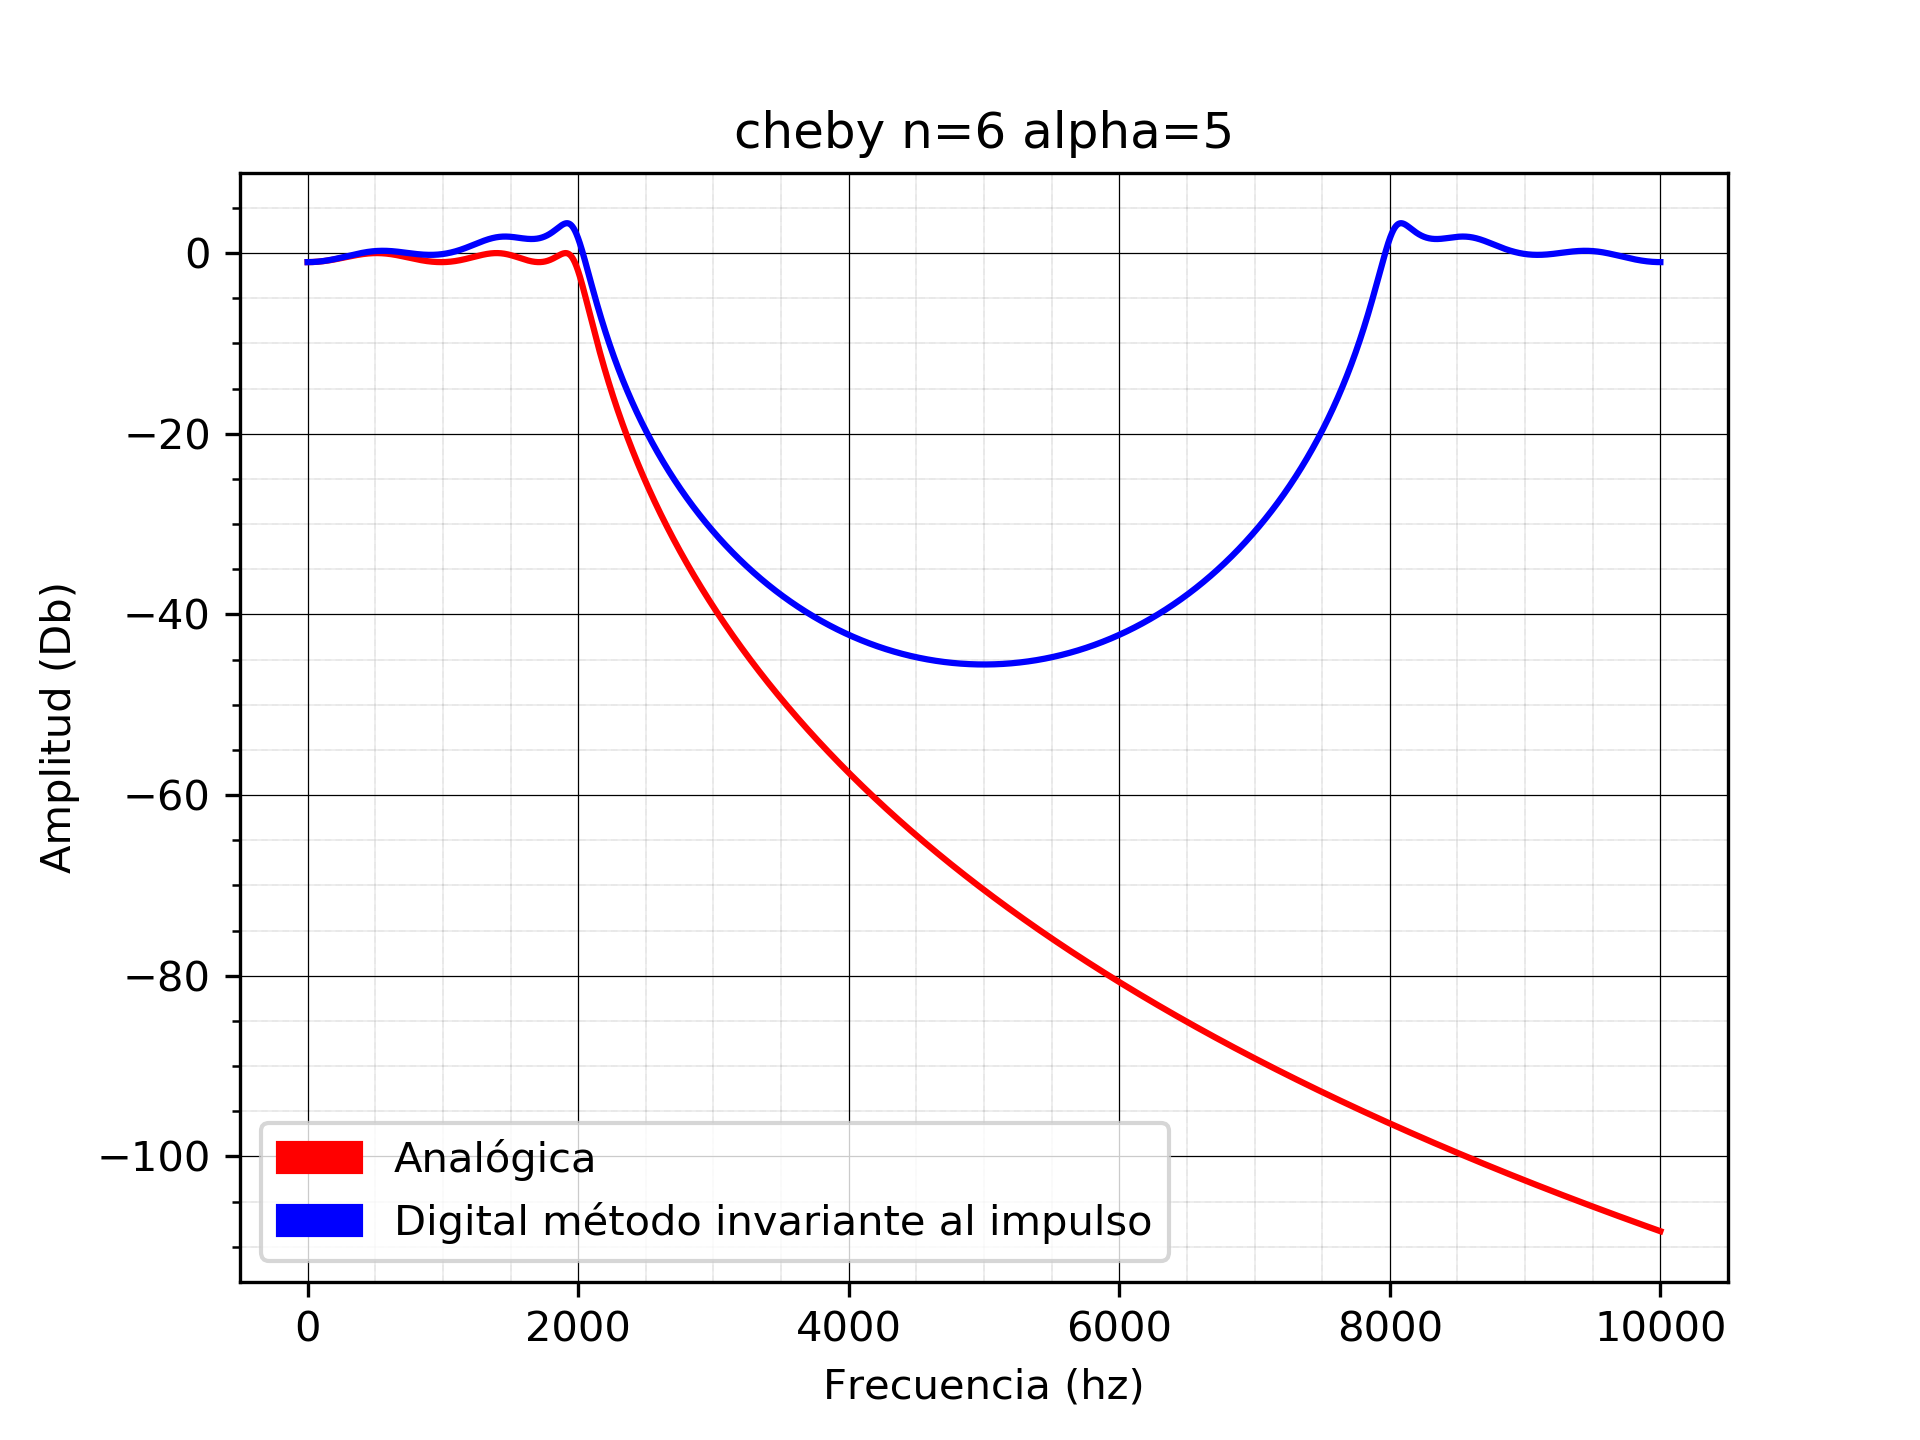
\includegraphics[scale=0.4]{output/cheby_matched_z/alpha=5/cheby_n=6.png}
	\caption{Ejemplo Cheby n=2, n=6 método matched Z}
	\label{fig:Caso 4}
\end{figure}

Con el filtro chebycheff no se observarón diferencias, la transformación se comporta de una forma similar con las dos aproximaciones

\section{Ejercicio 7}

\subsection{Método invariante al impulso}

Se repitió el ejercicio 6, pero ahora con $\alpha=8$. Esto significo una frecuencia de corte menor. A continuación se muestran los resultados


\begin{figure}[H]	
	\centering
	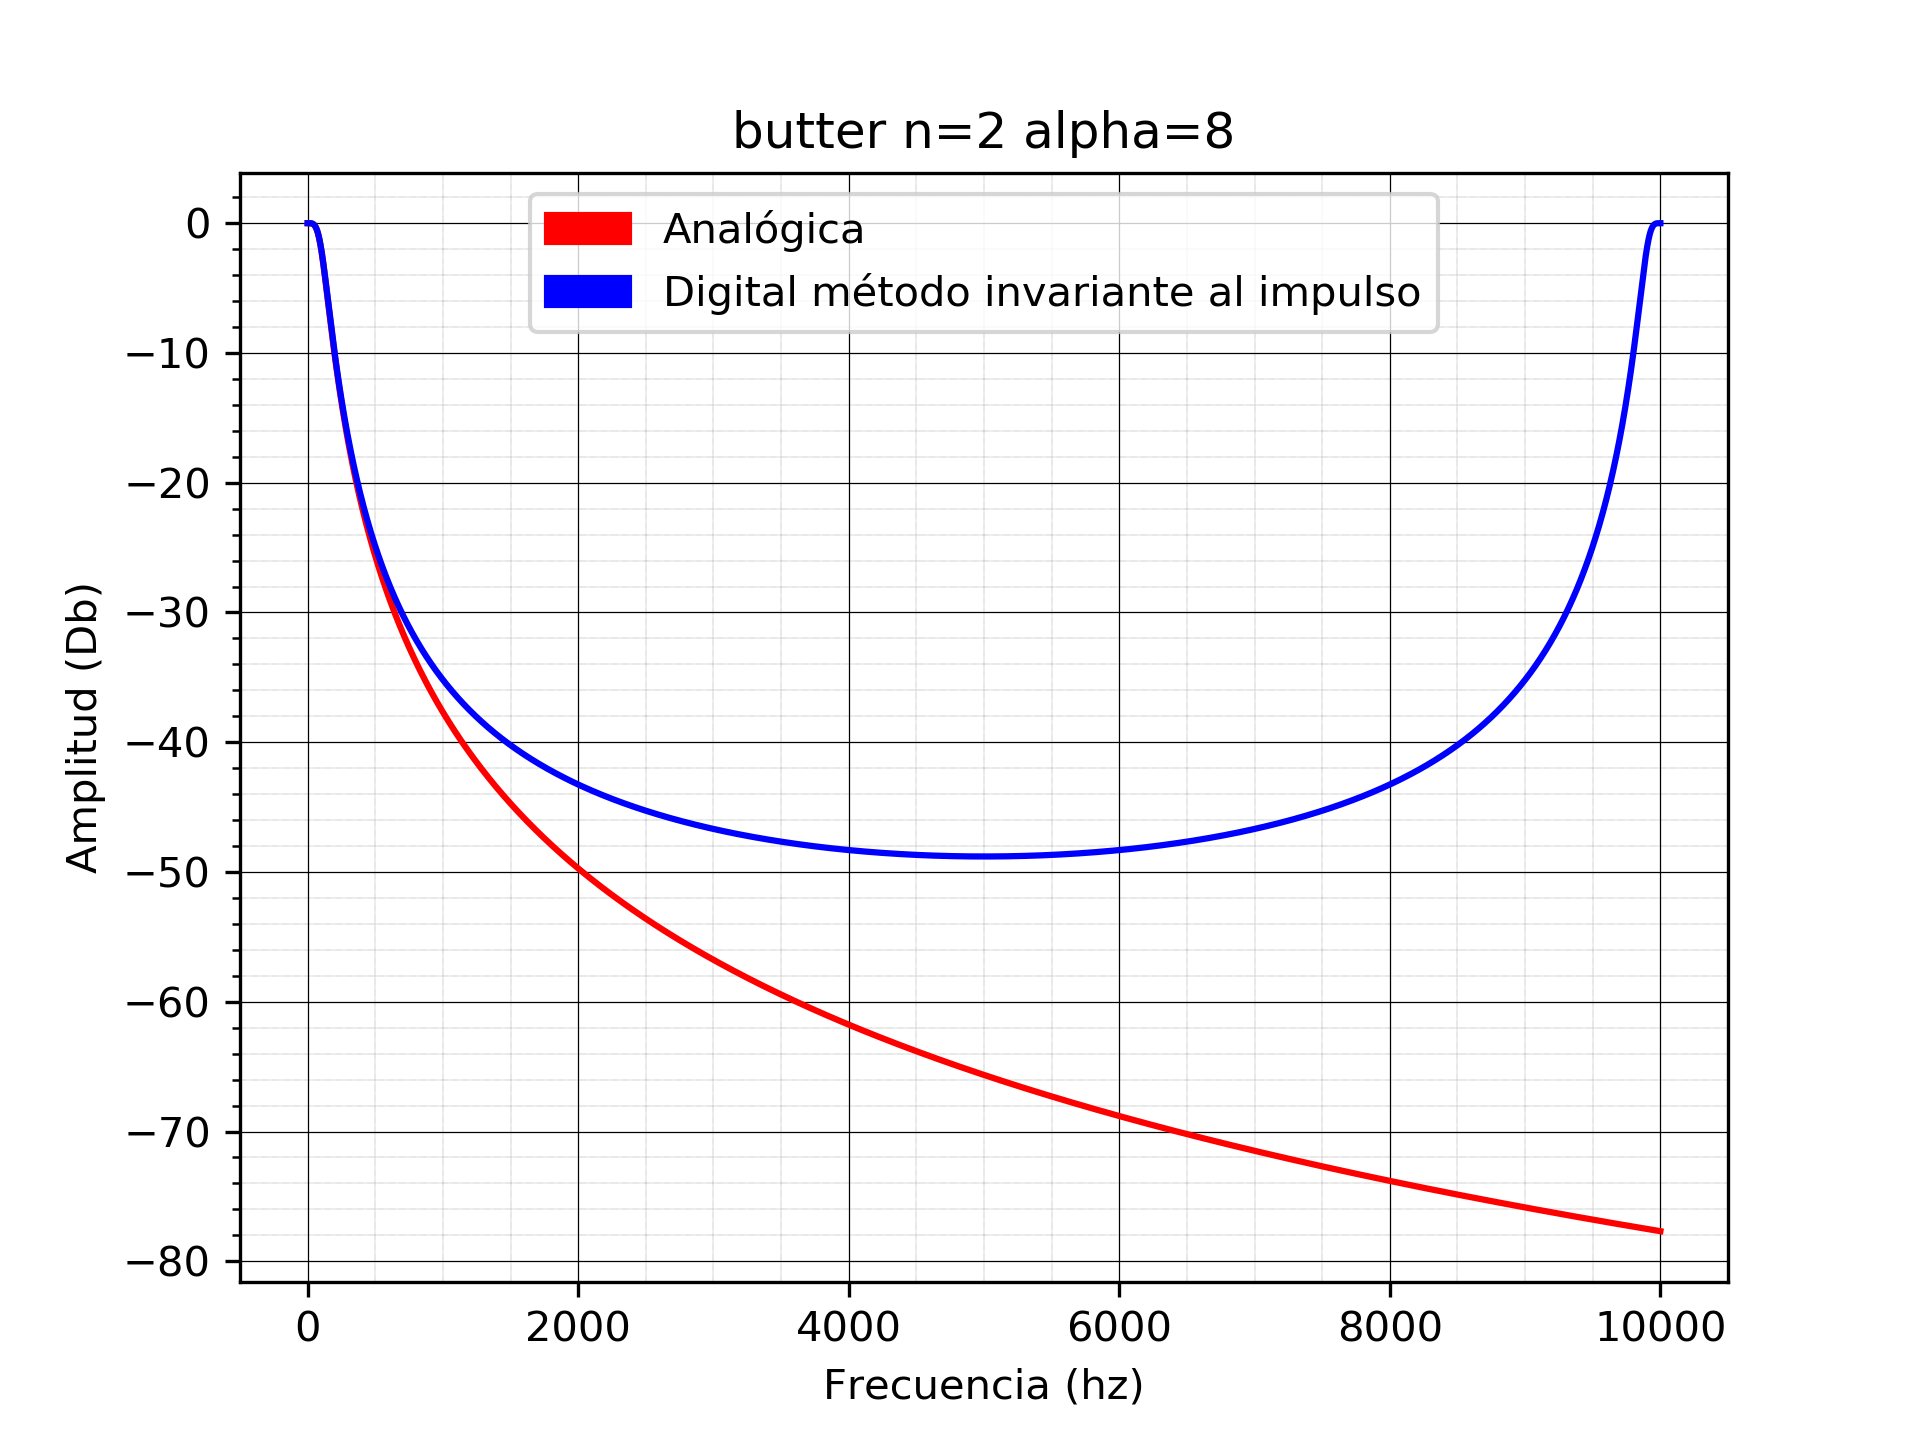
\includegraphics[scale=0.4]{output/butter/alpha=8/butter_n=2_alpha=8.png}
	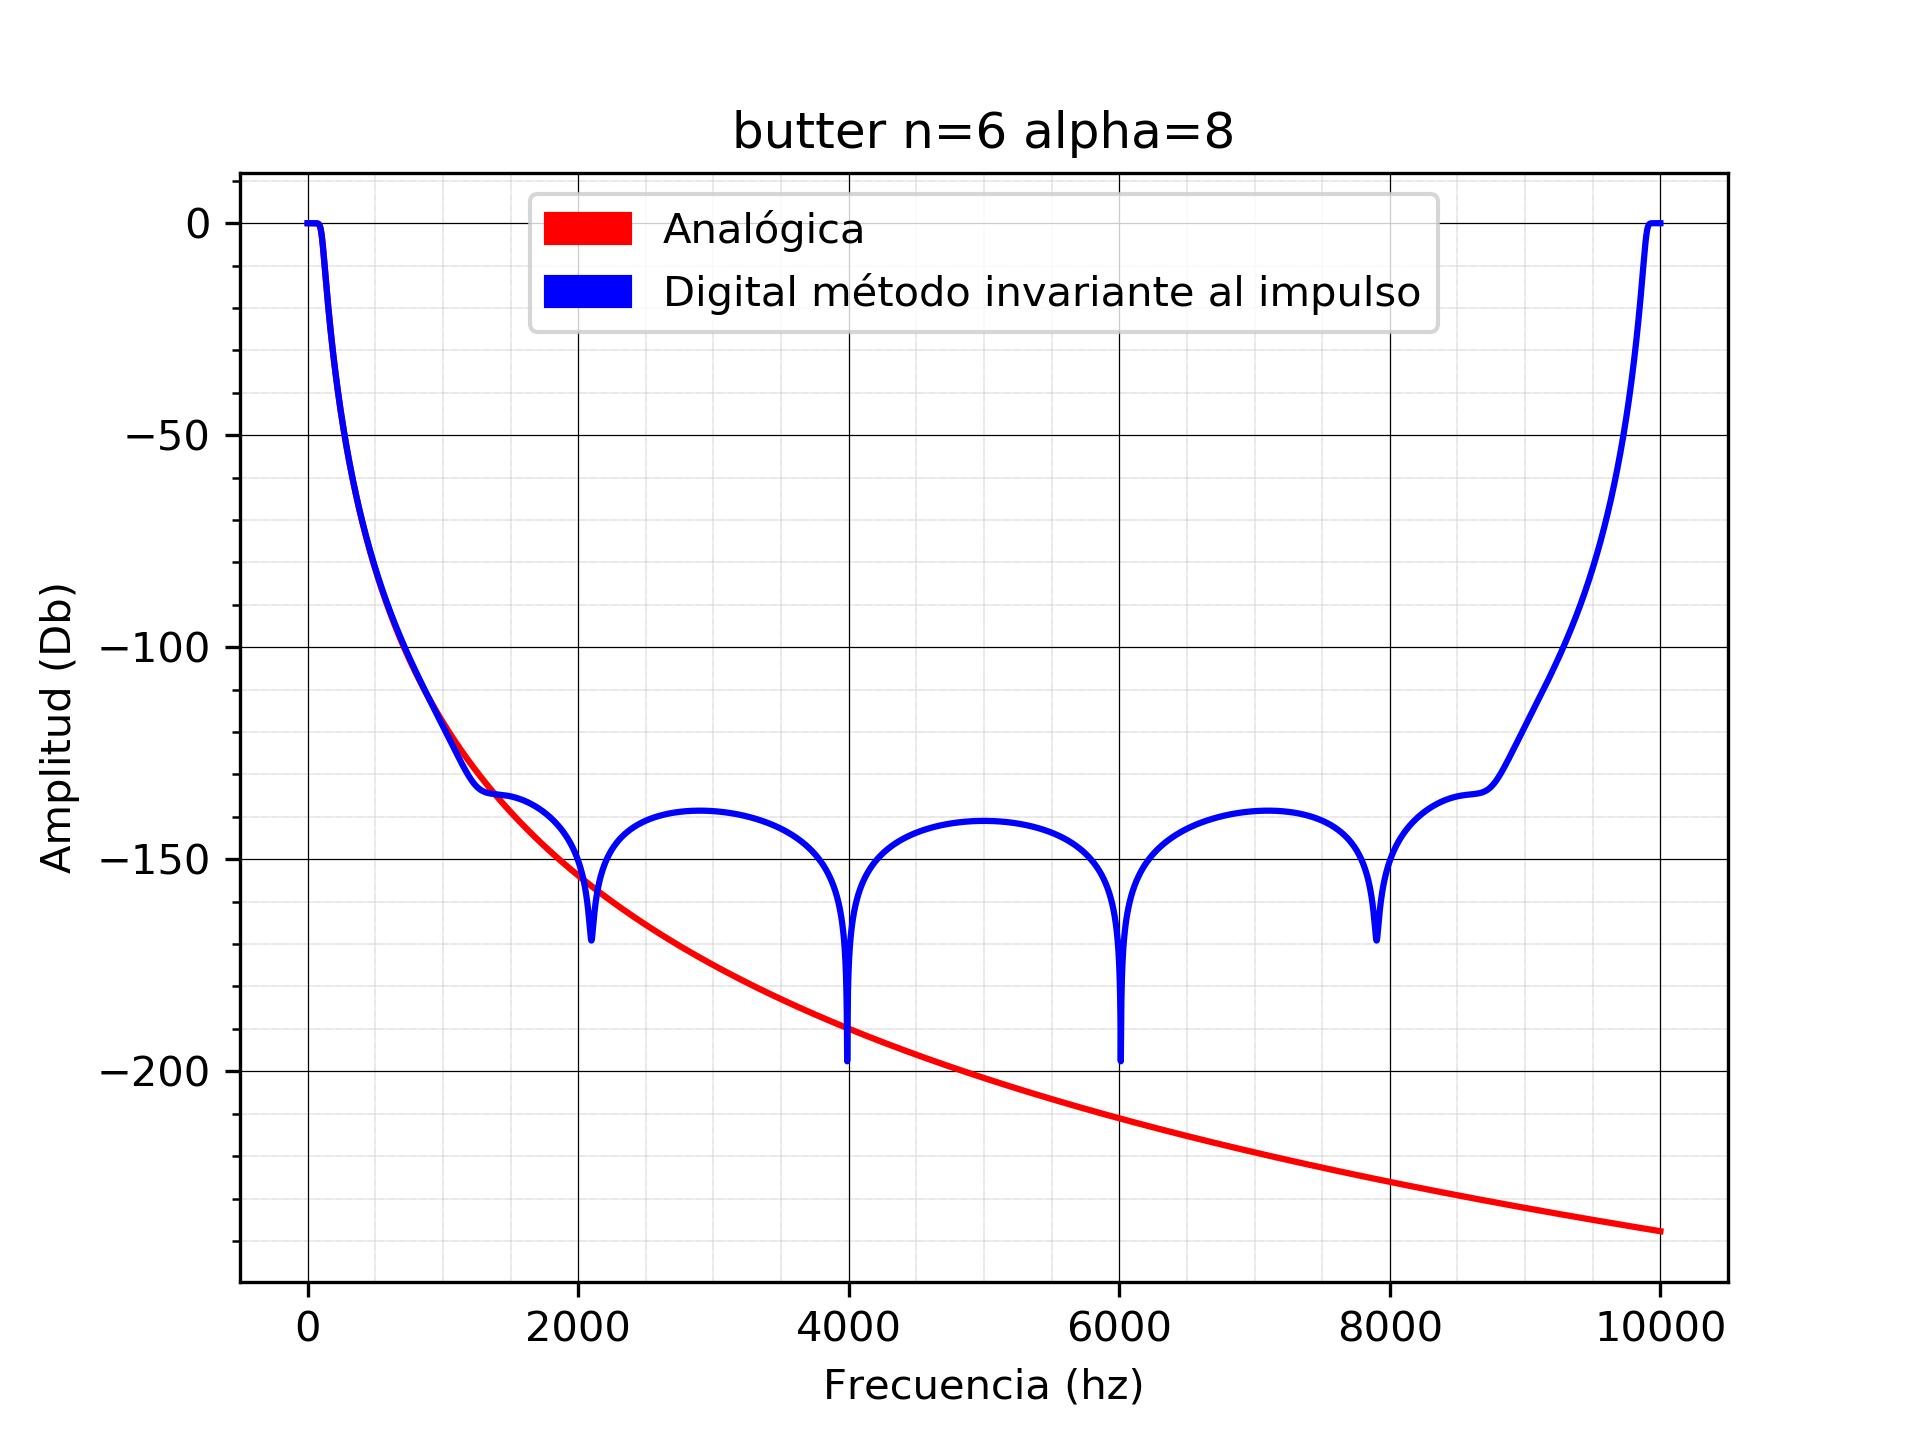
\includegraphics[scale=0.4]{output/butter/alpha=8/butter_n=6_alpha=8.png}
	\caption{Ejemplo Butter n=2, n=6 método invariante al impulso}
	\label{fig:Caso 5}
\end{figure}

\begin{figure}[H]	
	\centering
	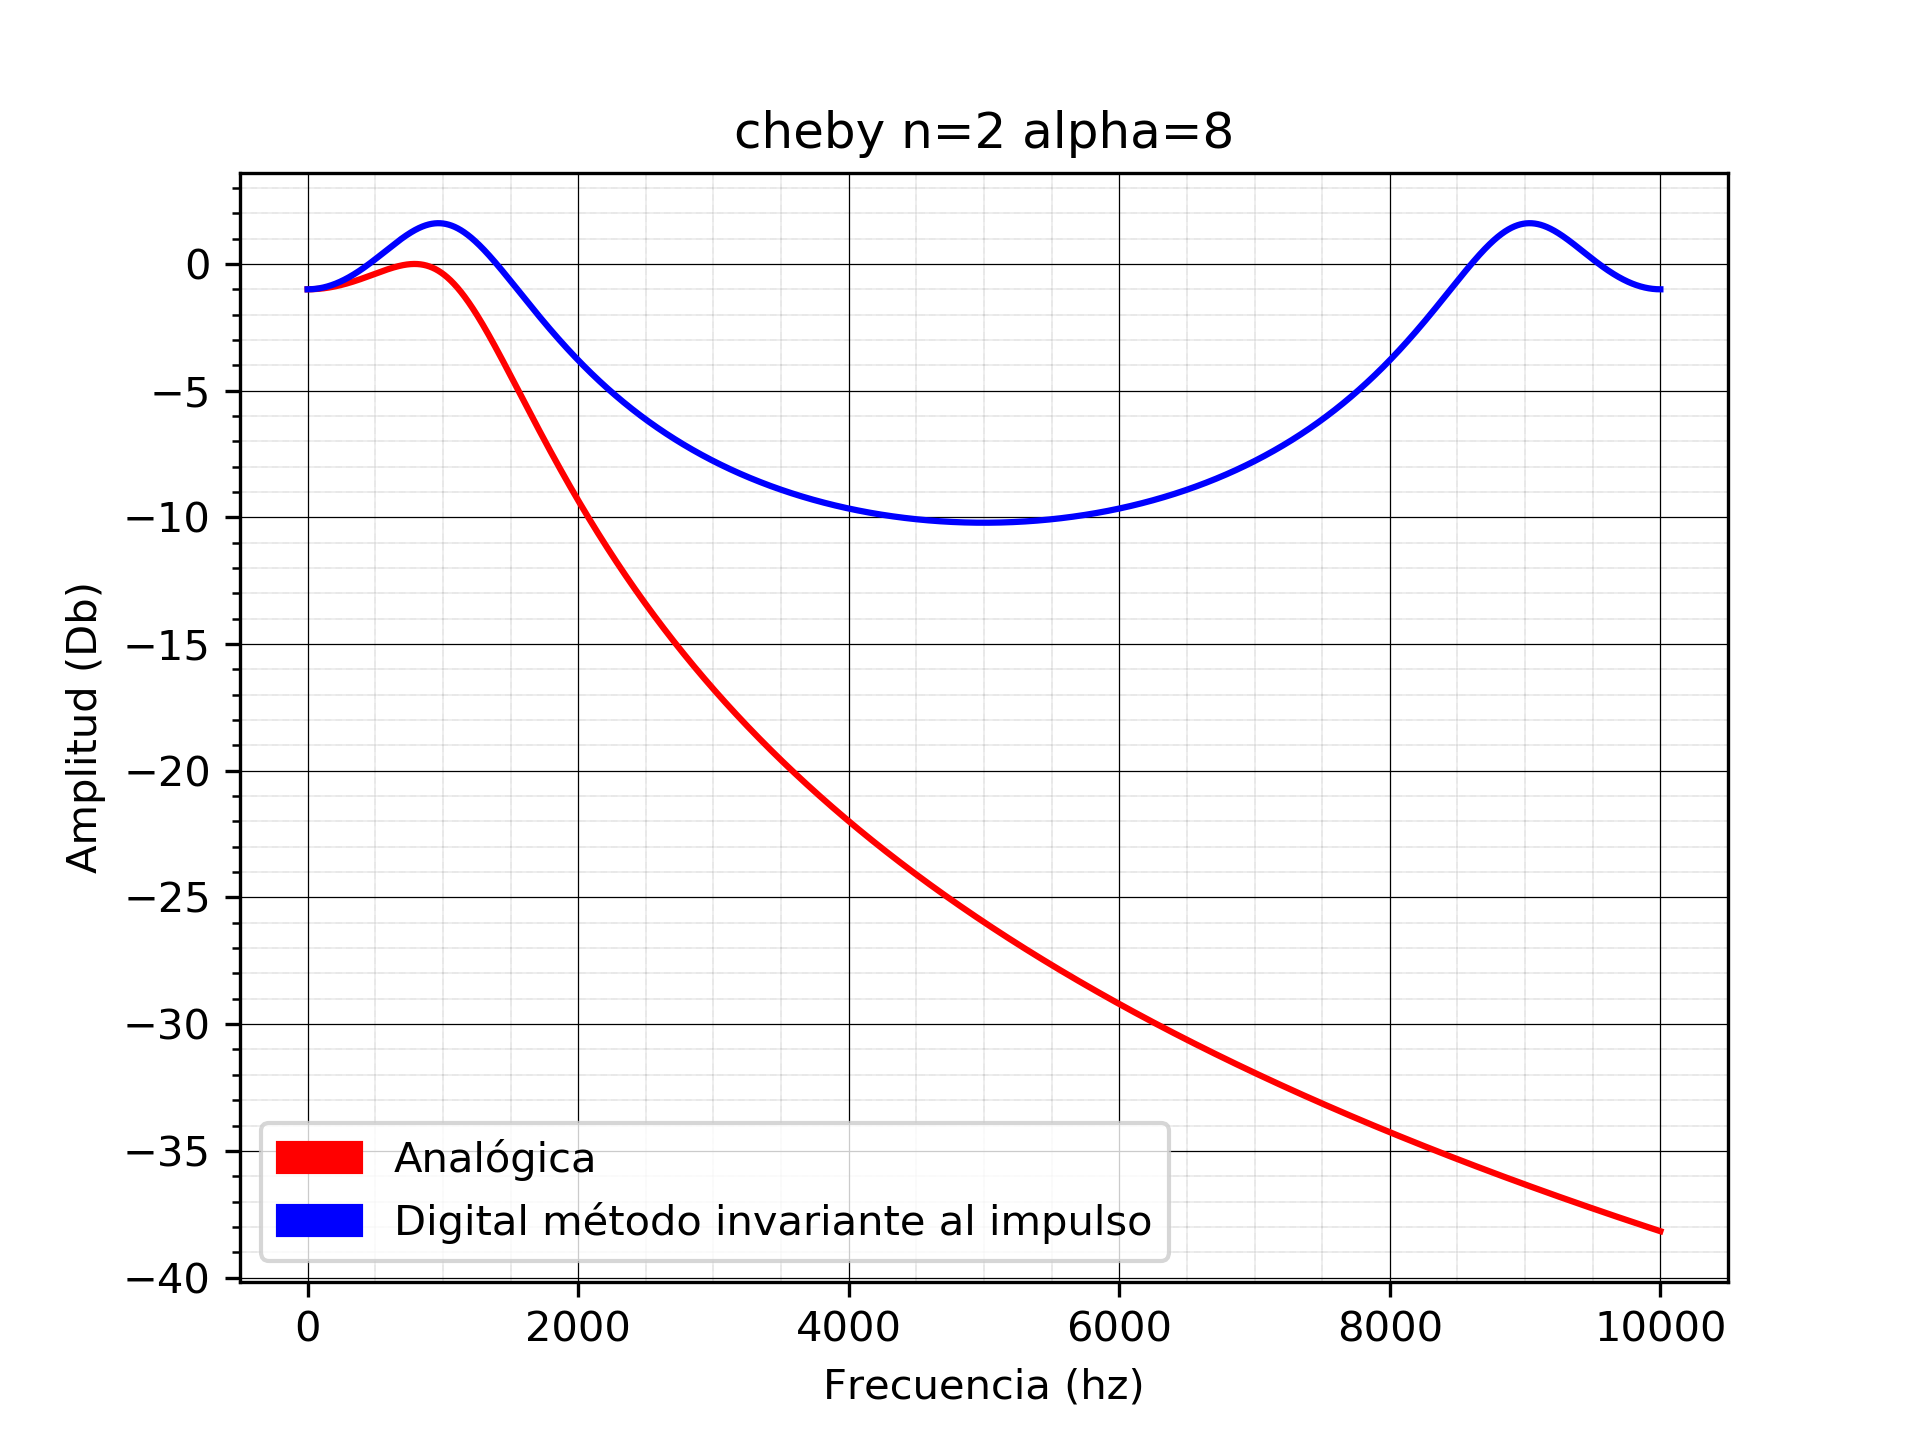
\includegraphics[scale=0.4]{output/cheby/alpha=8/cheby_n=2.png}
	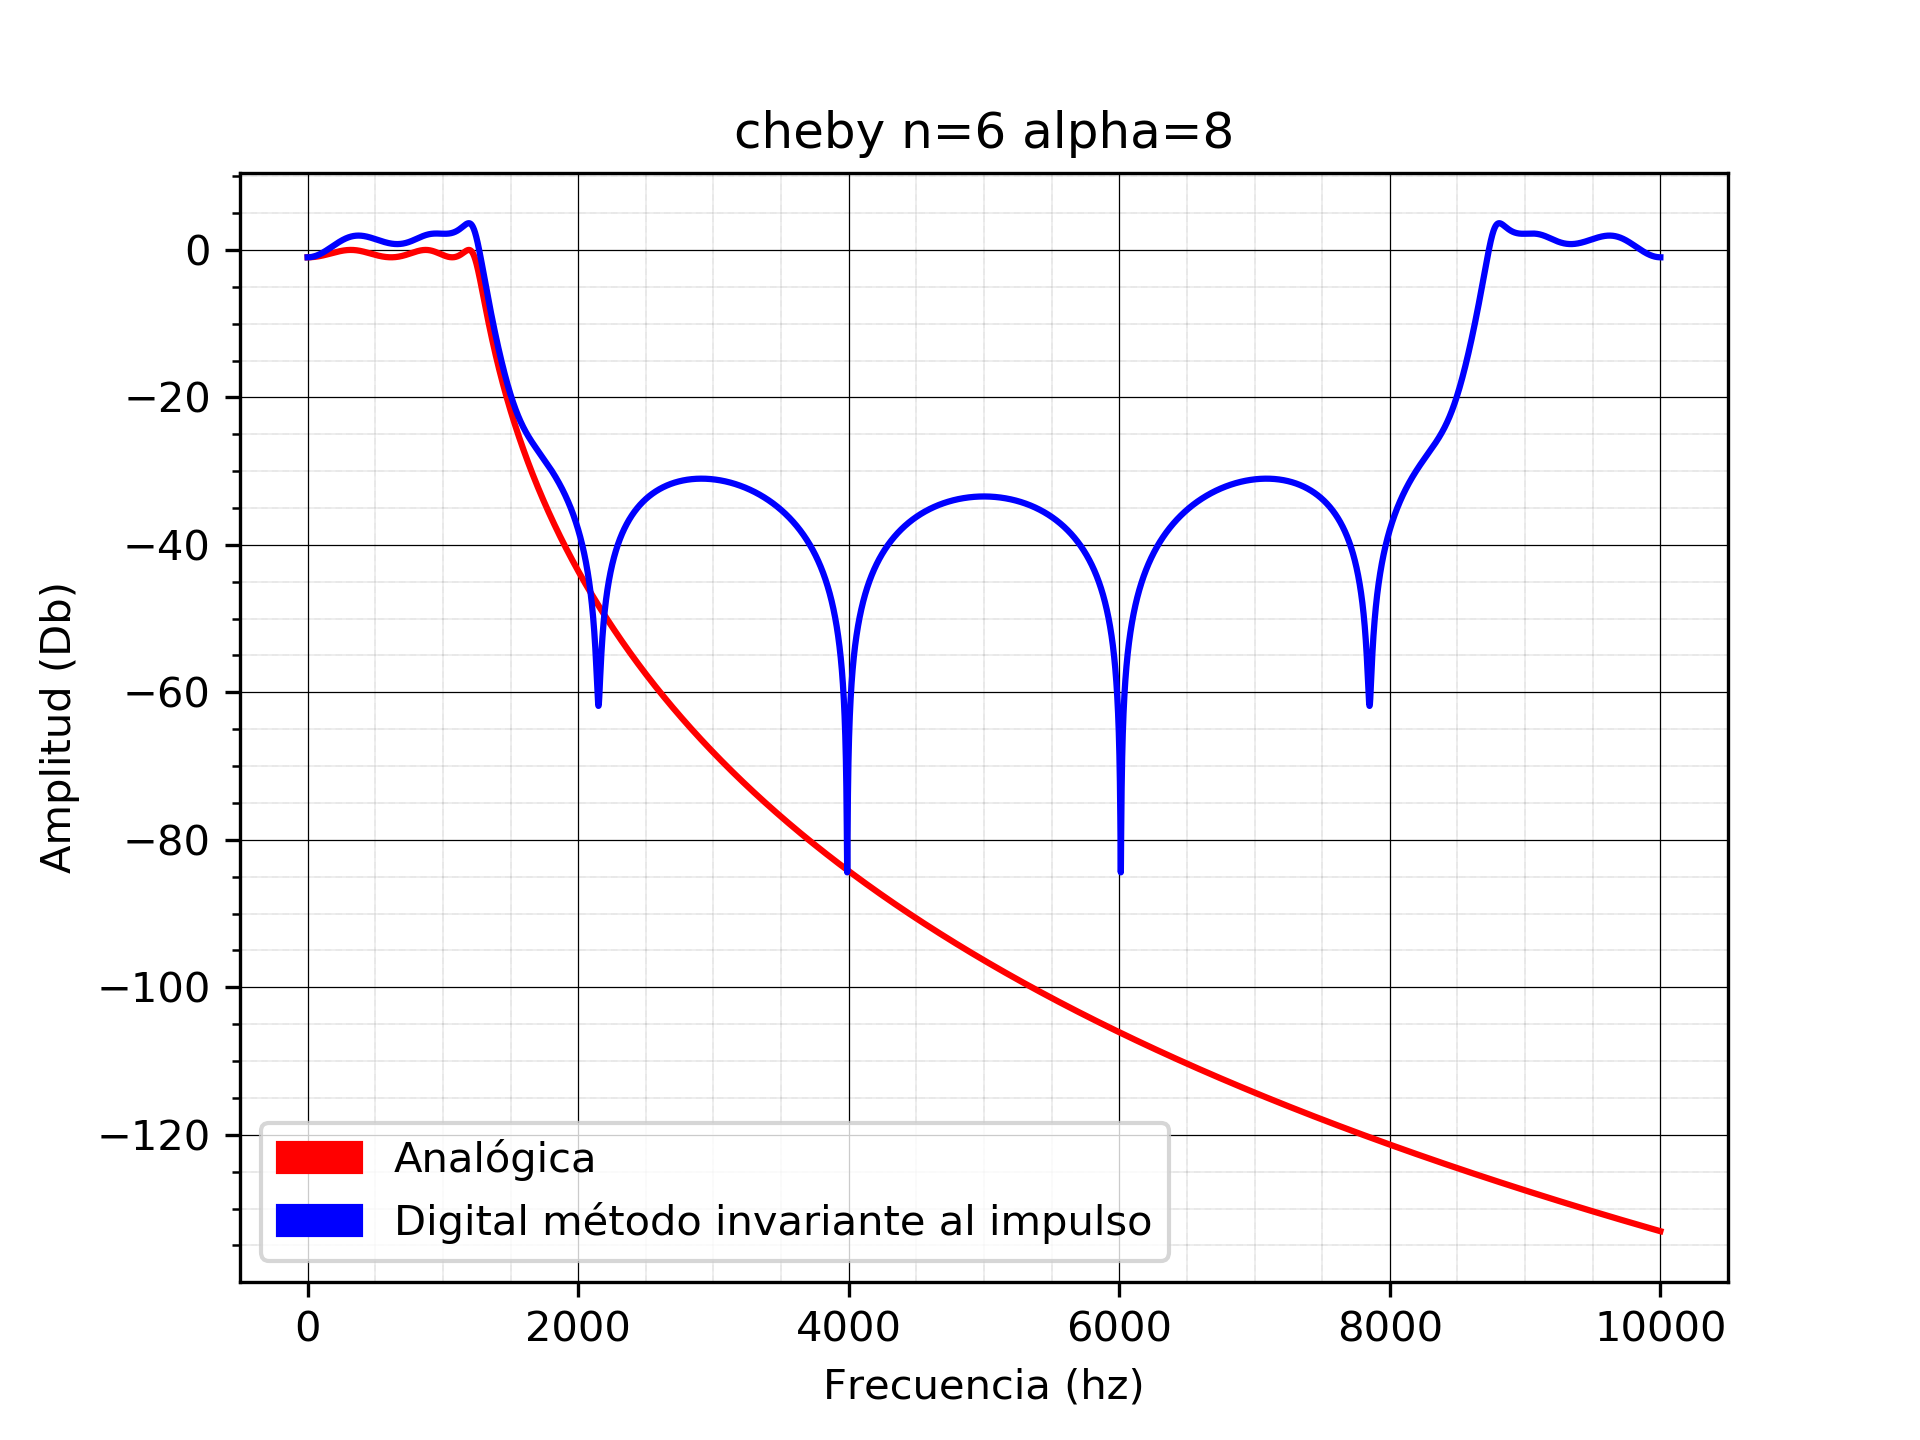
\includegraphics[scale=0.4]{output/cheby/alpha=8/cheby_n=6.png}
	\caption{Ejemplo Cheby n=2, n=6 método invariante al impulso}
	\label{fig:Caso 6}
\end{figure}


\subsection{Método matched Z}

\begin{figure}[H]	
	\centering
	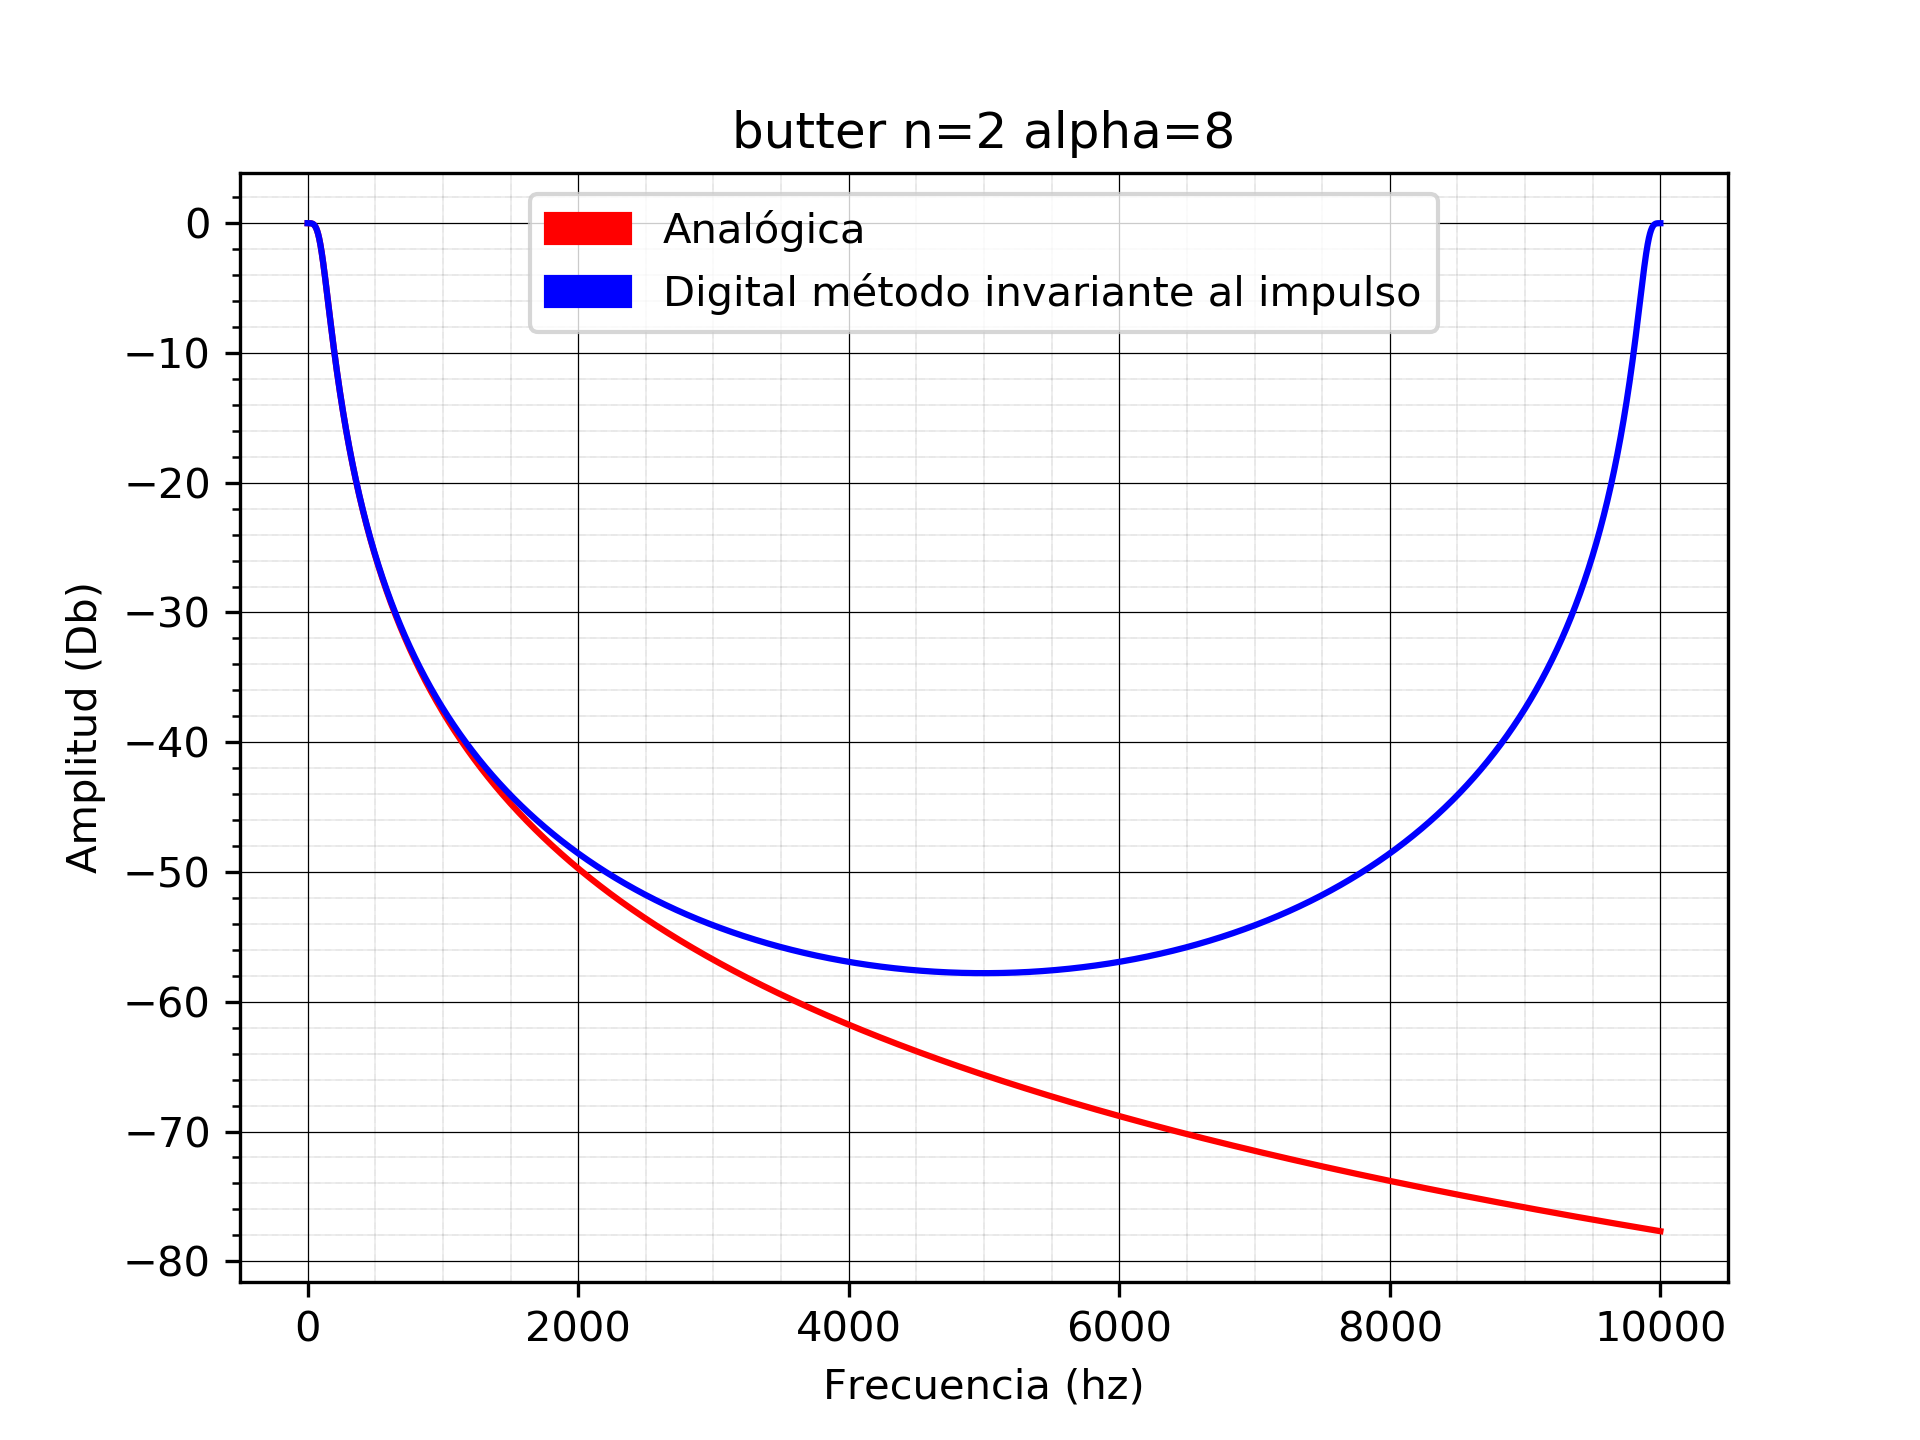
\includegraphics[scale=0.4]{output/butter_matched_z/alpha=8/butter_n=2_alpha=8.png}
	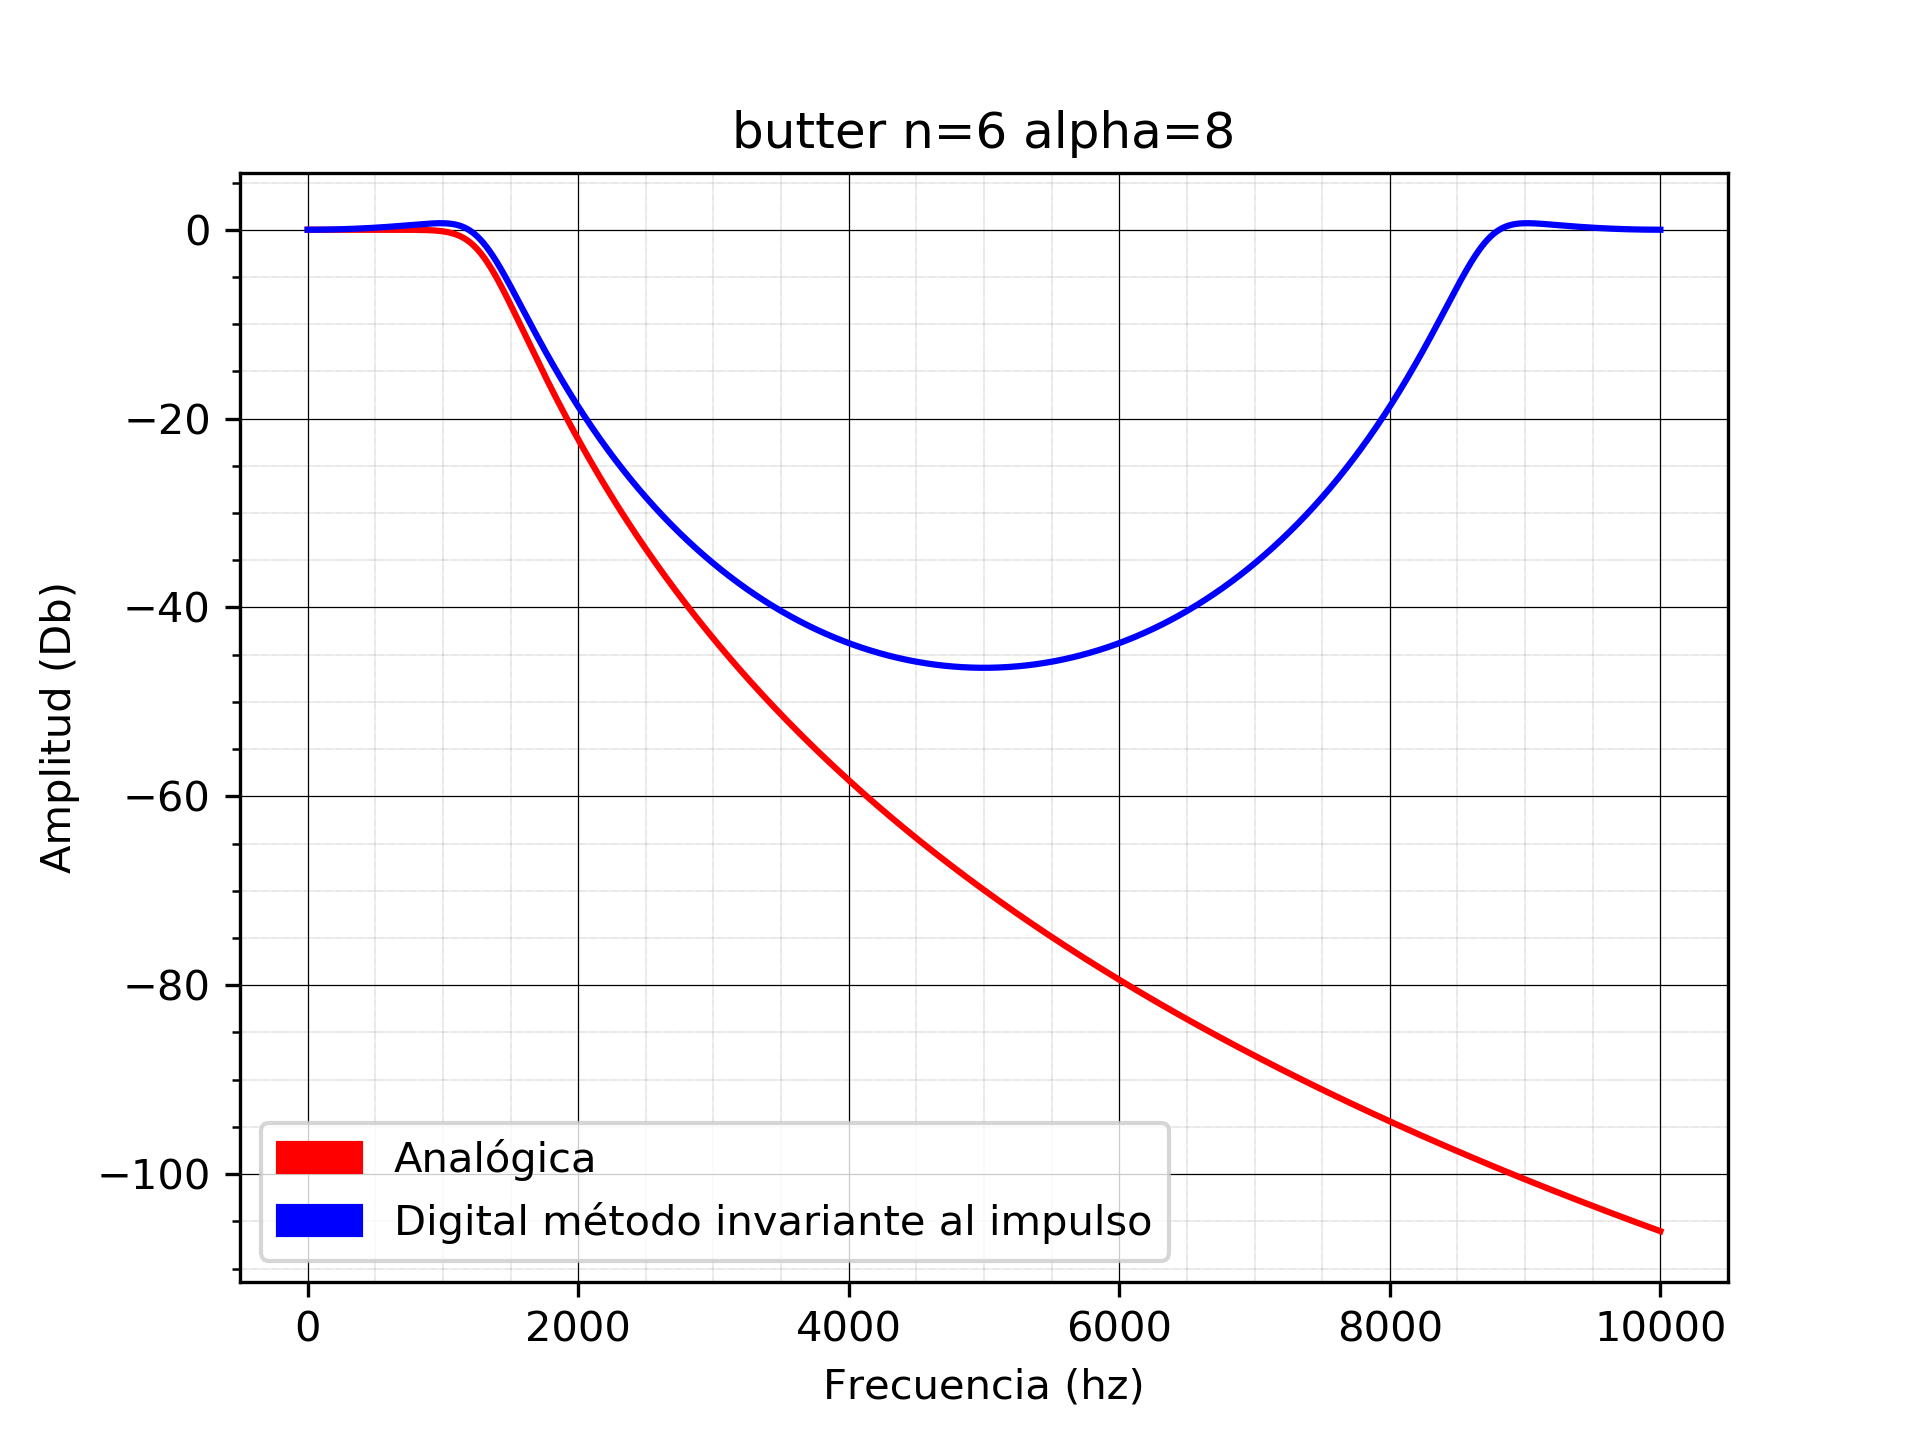
\includegraphics[scale=0.4]{output/butter_matched_z/alpha=8/butter_n=6_alpha=8.png}
	\caption{Ejemplo Butter n=2, n=6 método matched Z}
	\label{fig:Caso 5}
\end{figure}

\begin{figure}[H]	
	\centering
	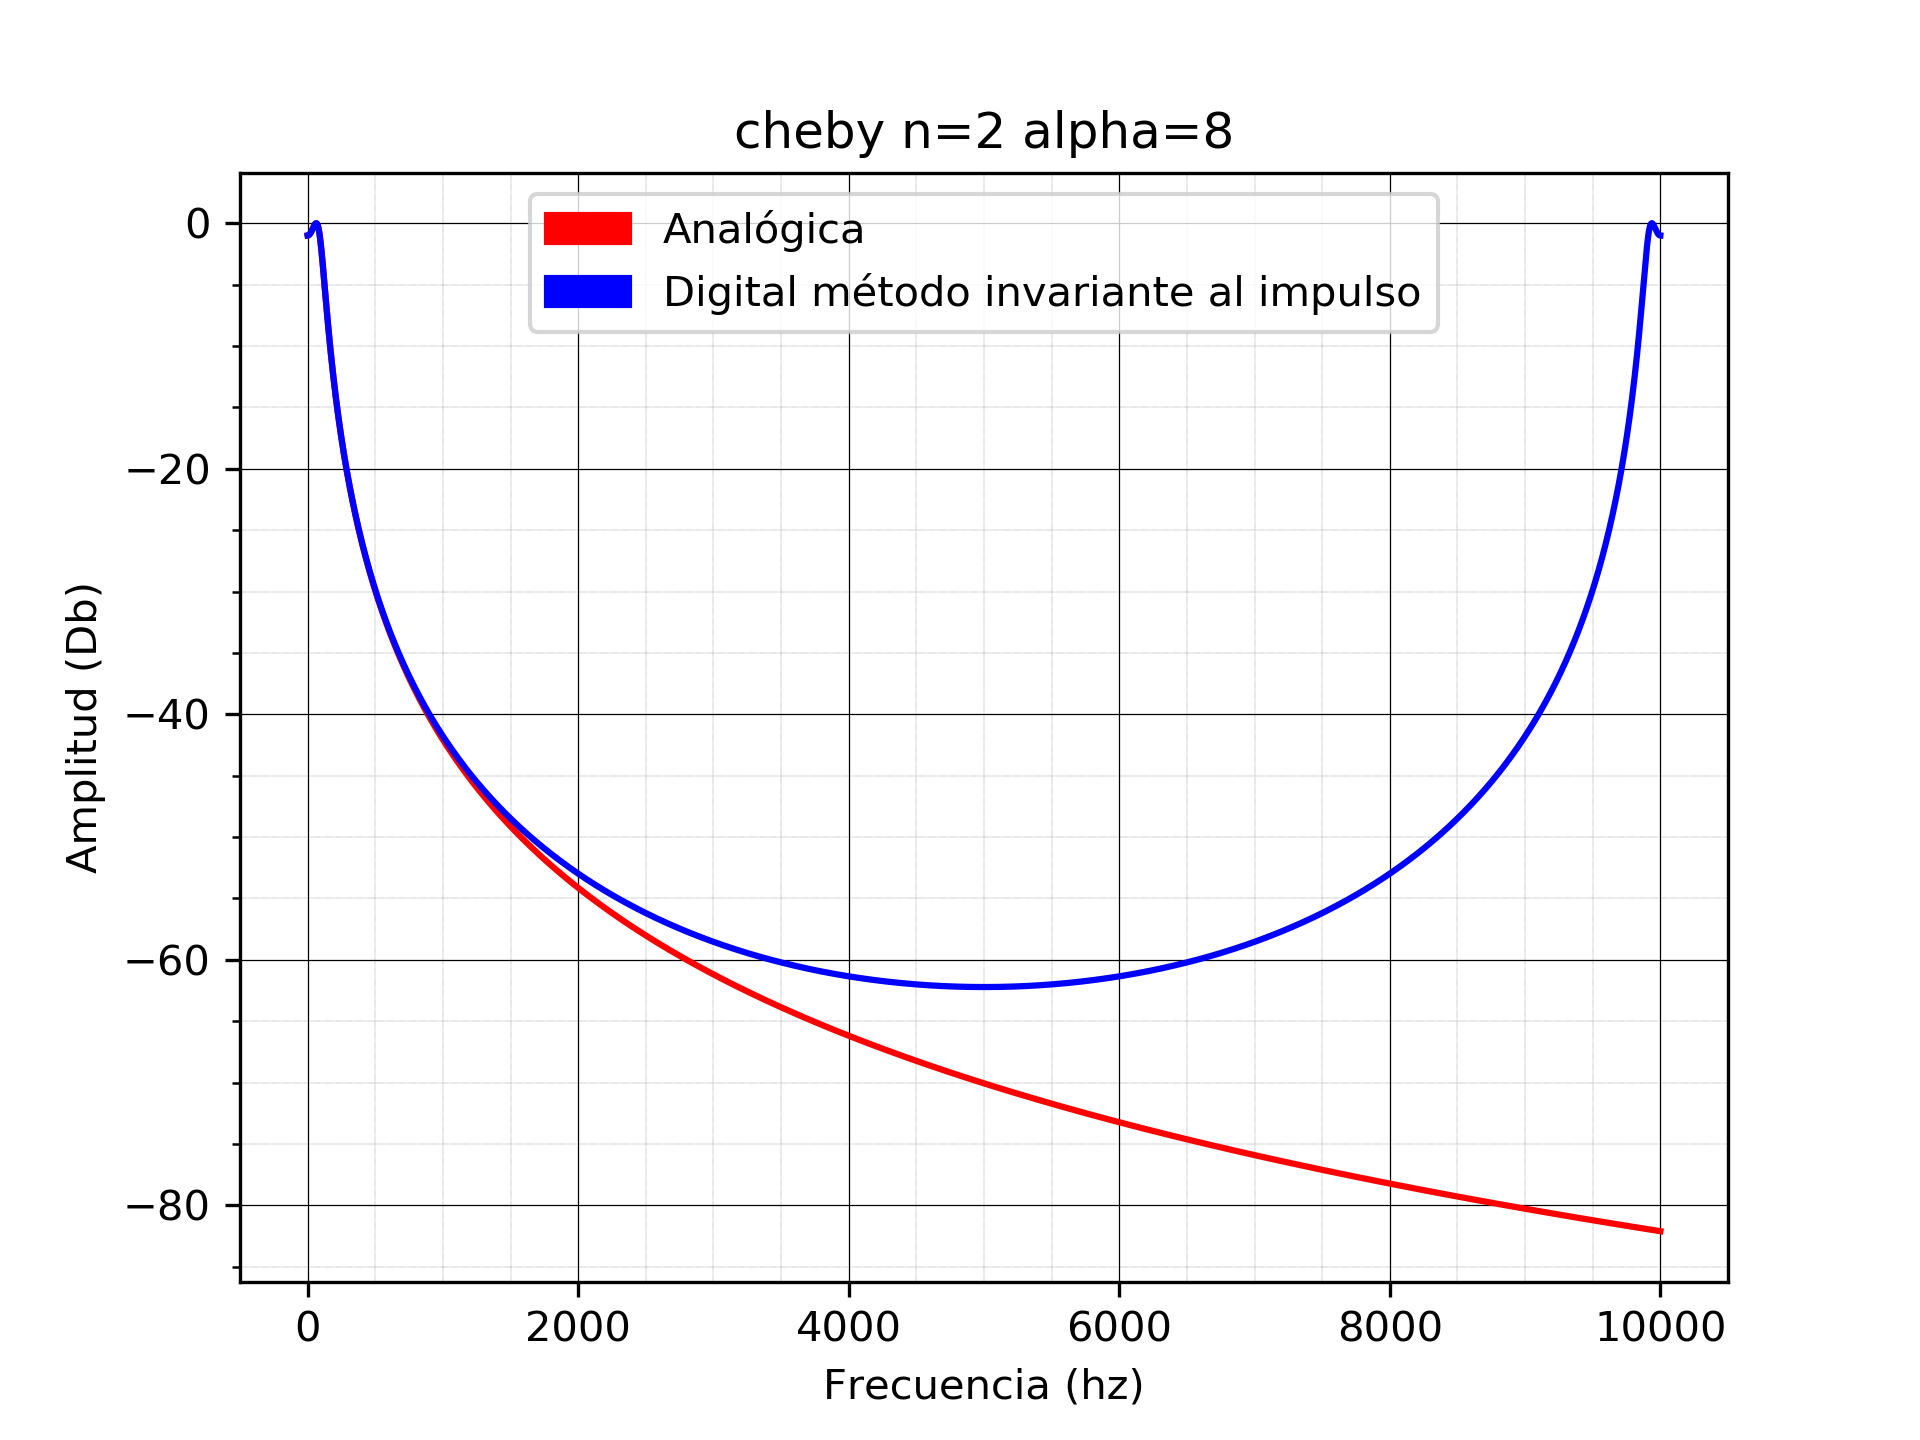
\includegraphics[scale=0.4]{output/cheby_matched_z/alpha=8/cheby_n=2.png}
	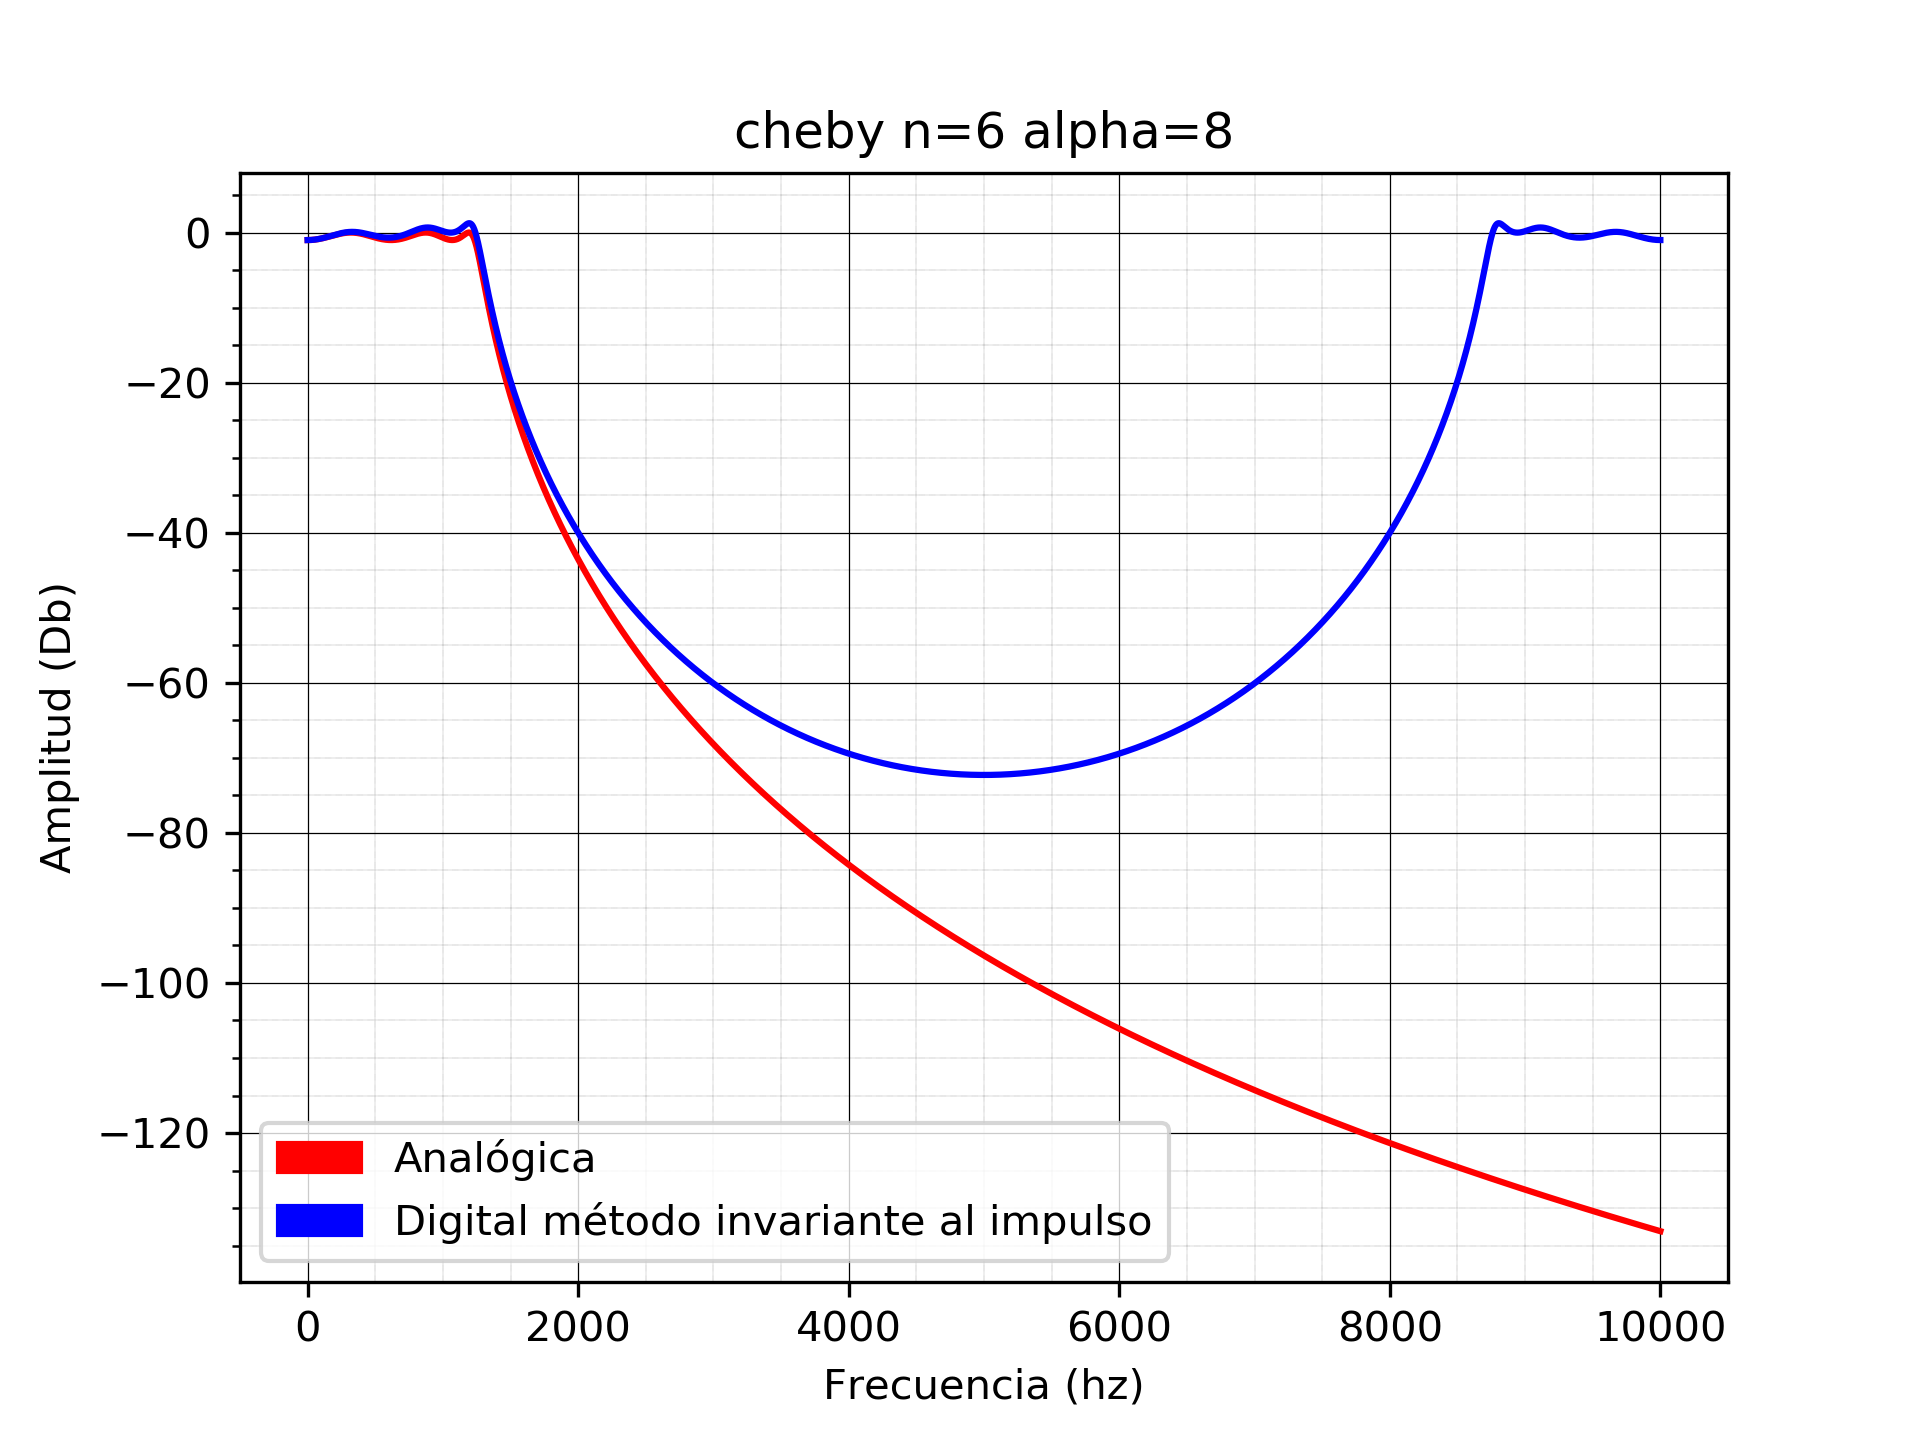
\includegraphics[scale=0.4]{output/cheby_matched_z/alpha=8/cheby_n=6.png}
	\caption{Ejemplo Cheby n=2, n=6 método matched Z}
	\label{fig:Caso 6}
\end{figure}

Como no se movió demasiado $f_p$ los resultados fueron similares, aunque, como se dimsminuyó en alguna medida $f_p$ hay que notar que fueron ligeramente mejores las transferencias, se ajustaron en una medida mayor a la transferencia analógica

\end{document}